\documentclass[12pt,fleqn]{report}
\usepackage{a4}
\usepackage{graphicx}
\graphicspath{ {./Figures/} }
\usepackage{psfrag}
\usepackage{amsmath}                     % \boldsymbol{#1}
\usepackage{amssymb}
\usepackage{Styles/hangcaption}
\usepackage{Styles/pstricks}
\usepackage{Styles/pst-node}
\usepackage{Styles/fancyheadings}
\usepackage{tocloft}
\usepackage{cite}
\usepackage{hyperref}
\usepackage[printonlyused]{acronym}
\usepackage{epstopdf}
\usepackage{advdate}
\usepackage[table, dvipsnames]{xcolor}
\usepackage{subfig}
\usepackage{float}
\usepackage{enumerate}
\usepackage{svg}
\usepackage{datetime}
\svgsetup{inkscapelatex=false}
\hypersetup{
    colorlinks=true,
    linkcolor=black,
    filecolor=black,      
    urlcolor=black,
    }
    
\newcommand{\yesthreeday}{{\AdvanceDate[-4]\today}}

\newdateformat{monthyeardate}{\monthname[\THEMONTH], \THEYEAR}
\epstopdfDeclareGraphicsRule{.pdf}{png}{.png}{convert #1\OutputFile}
\DeclareGraphicsExtensions{.svg,.png,.pdf}

%-----Tex width---------------------------------
\textwidth 16cm

%-----Line spacing-------------------------------
\renewcommand{\baselinestretch}{1.5}     % 1,1-zeilig

%---------Add dots in TOC-----------------------
\renewcommand{\cftsecleader}{\cftdotfill{\cftdotsep}}

%------Paragraph indention-------------------------------
\setlength{\parskip}{1.5ex plus0.5ex minus0.5ex}

%-----Prevent indent----------------------
\setlength{\parindent}{0em}

%-----Richtiger Abstand fur Einheiten-------------
\def\Unit{\hspace{0.25em}}

%-----Definition of the header--------------------
\pagestyle{fancyplain}
\renewcommand{\sectionmark}[1]{\markboth{Chapter~\thesection.~#1}{#1}}
\renewcommand{\subsectionmark}[1]{\markright{\thesubsection\ #1}}
\rhead[\fancyplain{}{\leftmark}]%
{\fancyplain{\thepage}{\thepage}} \cfoot{} \plainheadrulewidth
0.4pt
\makeatletter
\ifcase \@ptsize \relax % 10pt
  \addtolength{\headheight}{1\p@}
\or % 11pt
  \addtolength{\headheight}{2\p@}
\or % 12pt
  \addtolength{\headheight}{3\p@}
\fi \makeatother

%-----Equations / Figures / Tables numbering according to \ sections
\makeatletter
\renewcommand\theequation{\thesection.\arabic{equation}}
\renewcommand\thefigure{\thesection.\arabic{figure}}
\renewcommand\thetable{\thesection.\arabic{table}}
\@addtoreset{equation}{section} \@addtoreset{figure}{section}
\@addtoreset{table}{section} \makeatother

%-----Useful abbreviations----------------------
\newcommand{\mr}{\mathrm}
\newcommand{\bs}[1]{\mbox{$\boldsymbol{#1}$}}
\newcommand{\degree}[1]{\mbox{$#1^\circ$}}

%\renewcommand{\figurename}{Bild}

%------Bibliography style-----------------------
\bibliographystyle{IEEEtran}

%-----Aufzaehlunstiefe im Literaturverzeichnis---------------
\setcounter{tocdepth}{3}

\begin{document}
\pagenumbering{Roman}
\begin{titlepage}
  \begin{center}
      \vspace*{-4.0cm}
    \begin{figure}[!h]
\centering

\includegraphics[width=0.3\linewidth]{Figures/JKUAT_logo}
%\caption{}
\label{fig:jomologo}
\end{figure}
   \large{Jomo Kenyatta University of Agriculture and Technology}\\
    \large{College of Engineering and Technology}\\
    \large{School of Mechanical, Materials, and Manufacturing Engineering}\\
   \large{Department of Mechatronic Engineering}\\
    ------------------------------------------------------------------------------------------------\\
    \LARGE{\textbf{Design and Fabrication of a Prototype Mobile Platform with Holonomic and Omnidirectional Motion}}\\[0.5cm]
    \LARGE{\textbf{FYP-18-7}}\\[0.1cm]
    \LARGE{Interim Report}\\[0.1cm]
    \vspace{0.1cm}
    \large{\textbf{Gitu Kelvin Karimi (ENM221-0058/2017)}}\\
    \large{\textbf{Osodo Rodney David (ENM221-0091/2017)}}\\[0.3cm]
    \large{\textbf{Supervisor}}\\
    \large{Eng. Macben M. Makenzi}\\[0.2cm]
    % \vfill
    \large{\small{\monthyeardate\today}}\\
    \large{\small{Submitted in partial fulfilment of the requirements for the degree of Bachelor of Science in Mechatronic Engineering in Jomo Kenyatta University of Agriculture and Technology, 2022}}
    ------------------------------------------------------------------------------------------------\\[1.0cm]
  \end{center}
\end{titlepage}
%
%\pagenumbering{gobble}% Remove page numbers (and reset to 1)
\lhead{Declaration}
\addcontentsline{toc}{section}{Declaration}
\section*{Declaration}


We hereby declare that the work contained in this report is original; researched and documented by the undersigned students. It has not been used or presented elsewhere in any form for award of any academic qualification or otherwise. Any material obtained from other parties has been duly acknowledged. We have ensured that no violation of copyright or intellectual property rights has been committed.
\begin{enumerate}
	\item Gitu Kelvin Karimi\vspace*{.2cm}\\
	Signature\ldots\ldots\ldots\ldots\ldots\ldots\ldots\ldots\ldots\ldots Date\ldots\ldots\ldots\ldots\ldots\ldots\ldots\ldots\ldots\ldots
	\item Osodo Rodney David\vspace*{.2cm}\\
	Signature\ldots\ldots\ldots\ldots\ldots\ldots\ldots\ldots\ldots\ldots Date\ldots\ldots\ldots\ldots\ldots\ldots\ldots\ldots\ldots\ldots
\end{enumerate}

\vspace*{.5cm}
Approved by supervisor:
\begin{enumerate}
	\item Eng. Macben M. Makenzi\vspace*{.2cm}\\
	Signature\ldots\ldots\ldots\ldots\ldots\ldots\ldots\ldots\ldots\ldots Date\ldots\ldots\ldots\ldots\ldots\ldots\ldots\ldots\ldots\ldots
\end{enumerate}



\clearpage
\newpage
\lhead{Abstract}
\addcontentsline{toc}{section}{Abstract}
\section*{Abstract}
\label{sec:}

The vast majority of mobile platforms available today are non-holonomic. They only have one or two independent degrees of freedom. As a result, its manoeuvrability is limited, and it frequently requires a lot of space to perform functions like turning and parking. By increasing a vehicle's degrees of freedom and manoeuvrability, it can take various complex trajectories that non-holonomic vehicles find difficult or impossible to take.
\par
As a result, this project designs and develops a prototype mobile platform with holonomic and omnidirectional motion using castor wheels. Castors are used to move heavy loads in a variety of industries. Because castor wheels are difficult to control, we intend to introduce Direct Current Motors that will enable castor wheel control. The design will include the selection of Direct Current motors and power transmission systems based on the amount of power required to move heavy loads.
\par
The goal of this design is to give casters some form of control. This control will be accomplished by varying motor speed and direction, resulting in varying degrees of motion. This control will be accomplished remotely using hand motion control or a mobile application interface, depending on the application area. This will necessitate sophisticated software development, which will be accomplished through the use of high-level programming languages such as Python and Dart while leveraging low level capabilities to increase run time. 
\par
The goal is to have a prototype mobile platform capable of carrying a load of $40kg$ at the end of the design and fabrication process. This platform will not require manual control, but will instead be operated remotely via a mobile application software or hand motion control.

\clearpage
\lhead{Contents}
\tableofcontents
\clearpage
\addcontentsline{toc}{section}{Table of Contents}
\lhead{List of Figures}
\addcontentsline{toc}{section}{List of Figures}
\let\oldnumberline\numberline%
\renewcommand{\numberline}{\figurename~\oldnumberline}%
\listoffigures
\clearpage
\lhead{List of Tables}
\addcontentsline{toc}{section}{List of Tables}
\listoftables
\newpage
\clearpage
\lhead{Nomenclature}
\addcontentsline{toc}{section}{Nomenclature}
\linespread{1.0}
\setlength{\parskip}{0.5em}
\section*{Nomenclature}
% Some text \ac{USA}

% ARRANGE IN ALPHABETICAL ORDER
\begin{acronym}
 \acro{AC}{Alternating Current}
 \acro{API}{Application Programming Interface}
 \acro{BJT}{Bipolar Junction Transistor}
 \acro{COAP}{Constrained Application Protocol }
 \acro{DAC}{Digital to Analogue Converter}
 \acro{DC}{Direct Current}
 \acro{LIDAR}{Light Detection and Ranging}
 \acro{MOSFET}{Metal Oxide Silicon Field Effect Transistors}
 \acro{MQTT}{MQ Telemetry Transport}
 \acro{PWM}{Pulse Width Modulation}
 \acro{RPM}{Revolutions Per Minute}
 \acro{SDG}{Sustainable Development Goals}
 \acro{SLAM}{Simultaneous Localisation and Mapping}
 \acro{SMPS}{Switched Mode Power Supply}
 \acro{UN}{United Nations}
 \acro{MCU}{Microcontroller Unit}
 \acro{IMU}{Inertial Measurement Unit}
\end{acronym}

\clearpage
\newpage

\pagenumbering{arabic}
  \lhead{Chapter 1. Introduction}
  \chapter{Introduction}
\newcommand{\sectionbreak}{\clearpage}

\label{sec:introduction}
\section{Background}
Mobile robots are increasingly being used in non-industrial applications such as military, disaster relief, and home automation. One way to classify mobile robots is based on their type of motion, which can be either holonomic or non-holonomic. Holonomic mobile vehicles have the advantage of being controllable by degrees of freedom equal to the mobile robot's total degrees of freedom. A mobile robot classified as omnidirectional, on the other hand, can change the direction of motion without performing intermediate rotation steps and can move in all directions from a given starting point while simultaneously rotating. This project will attempt to apply the concepts of omnidirectional and holonomic motion to a set of wheels in order to create a mobile platform with industrial applications. The wheels under consideration are castor wheels, which are commonly found in homes, industrial plants, warehouses, and other large objects that require mobility.

\section{Problem statement}

Mobile robots and platforms have found widespread use in homes and other non-industrial settings. These vehicles are mostly unmanned and are controlled remotely. This technology can be used in the industrial application of casters. On the other side, casters are used on the warehouse or factory floor to move heavy and large objects. This is a manual process in which the operator physically pushes the caster around. The next step is to remove manual control and remotely control the caster wheels.
\par
Despite this being the obvious next step, caster wheels in the industry currently require manual control. Casters require an initial push force to begin rolling. Other applications of caster wheels such as shopping trolleys and hospital beds also require manual control. 
\par
The current implementation of caster wheels defies the trends in technological innovation being observed in the world. Maintaining manual control on casters is less efficient compared to an automated version. Furthermore, labourers get tired easily when pushing the heavy casters around especially due to difficulty in maintaining the correct swivelling. The need, therefore, arises to develop a controllable version of castor wheels so that the process can be automated.

\section{Objectives}

\subsection{Main objective}

To design and fabricate a prototype mobile platform capable of omnidirectional and holonomic motion.

\subsection{Specific objectives}

\begin{enumerate}
	\item To design and build a mechanical chassis and frame that will hold the wheels, power transmission unit and carry the load respectively \vspace*{.2cm}
	\item To design and construct a power transmission that transmits power from the motor to the wheel shaft unit\vspace*{.2cm}
	\item To design a \ac{DC} motor control circuit for individual caster wheels\vspace*{.2cm}
	\item To develop  algorithms to control the motors and achieve simultaneous holonomic motion from the caster wheels and remotely control the mobile platform\vspace*{.2cm}
	
\end{enumerate}

\section{Justification of the study}
The apparent availability of low-cost and easily accessible technologies that bridge the gap between nonholonomic and holonomic motion control motivates us to conduct this research. Navigation to and from tight spaces is possible with holonomic motion. Furthermore, developing a low-cost holonomic mobile platform in the field of mobile robots, particularly in Sub-Saharan Africa, aligns with one of the \ac{UN} \ac{SDG} goals of infrastructure development, inclusive and sustainable industrialisation, and innovation \cite{noauthor_goal_nodate}.
This is where the world is going, and it is only natural for us to try to follow suit.

\section{Expected Outcomes}
At the end of the design process, we expect to come up with the following:
\begin{enumerate}
    \item A mobile platform that can move a maximum payload of $40kg$
    \item A mobile platform that can move in any direction without whilst carrying a load
    \item A hand motion controller that can be able to control the mobile platform remotely
    \item A mobile application that can be able control the mobile platform remotely
\end{enumerate}
  \clearpage
  \lhead{Chapter 2. Literature Review}
  \chapter{Literature Review}
\label{sec:review}
% \newcommand{\sectionbreak}{\clearpage}
\section{Introduction}
The vast majority of mobile platforms and unmanned vehicles currently in use are non-holonomic \cite{sanchez-orta_aerial_2020}. They only have one or two independent degrees of freedom. As a result, its manoeuvrability is restricted, and it frequently necessitates a large amount of space to control functions like turning and parking \cite{bremer_problems_2010}. This is visible when a car wants to turn $180^0$. We improve a vehicle's manoeuvrability by increasing its degrees of freedom. It can take many complex paths that conventional nonholonomic vehicles find difficult or impossible to follow. The relationship between a robot's controllable and total degrees of freedom is referred to as holonomic \cite{yun_unified_1998}. Any mobile platform with three independent degrees of freedom in a plane is referred to as a holonomic platform. The robot is said to be holonomic if the controllable degree of freedom equals the total degree of freedom \cite{thompson_chapter_2017}. In contrast to car-type vehicles, which must turn or change orientation when moving, independent degrees of freedom indicates that it can change its orientation or position without affecting other motions. A holonomic drive is demonstrated by a robot built on castor wheels or Omni-wheels, which can freely move in any direction and has controllable degrees of freedom equal to total degrees of freedom.

\subsection{Mobile Platforms}
Researchers have been working on omnidirectional wheeled mobile robots for the last three decades. There are also legged mobile robots that can move in both omnidirectional and holonomic directions. Legged mobile platforms have the advantage of being highly adaptable to uneven terrain, having low soil interaction, and being able to perform tasks in congested and narrow areas. Despite this, their slow mobility, low payload-to-mechanic weight ratio, and complex design and control make them difficult to locate.

\subsection{Caster wheel}
A castor or caster wheel is a relatively free-rolling ,not powered, small undriven wheel. They are designed to be attached to the bottom of a larger object, to enable easy movement across a floor or other hard surface. Castor wheels are manufactured in either a single-wheel, double-wheel, or compound-wheel configuration.
\par
Most castors are used simply to make a heavy or cumbersome piece of furniture or machinery - the vehicle - easier to move. Affixing small, unobtrusive wheels to the bottom of any large or bulky item is a great way to make it more mobile in certain scenarios. In most cases, they are attached to the underside of the vehicle via a fixed top plate, from which the wheel assembly hangs.
\par
When choosing the type of casters to use in an application, weight considerations need to be considered depending on the load the casters will be required to move. To achieve this, we need to consider the weight of the item being supported as shown by equation \ref{eq:1}.

\begin{equation} \label{eq:1}
total\:load\:capacity = individual\:weight\:rating * number\:of\:wheels
\end{equation}

The total load-bearing capacity of your castors should always be at least 30\% higher than the total weight of the item when fully loaded, to give a sufficient safety margin. Another consideration to take into account is the type of surface the castors will be moving on. These surfaces are either flat and smooth that can accommodate small wheels or rougher surfaces that require wheels with larger diameters.
\par
There are several types of caster wheels each suited to a different application. The most common casters are shown in Figure \ref{fig:casterwheels}
\vspace{5mm}
\begin{figure}[H]
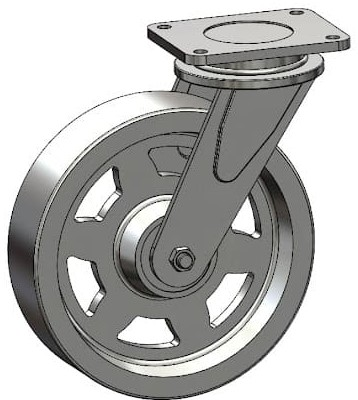
\includegraphics[scale=0.45]{Figures/ferrous-caster-wheel.jpg} 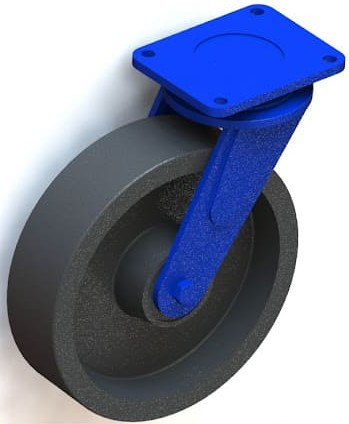
\includegraphics[scale=0.45]{Figures/synthetic-tread-wheels.jpg} 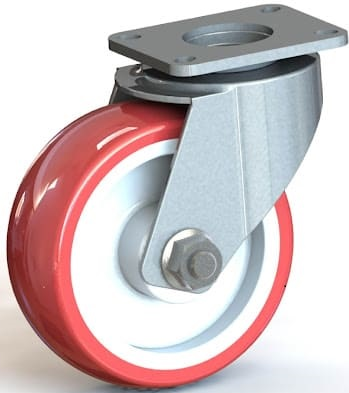
\includegraphics[scale=0.45]{Figures/polyurethane-caster-wheel.png}\centering
\caption[Caster Wheels] {Caster Wheels \cite{noauthor_caster_nodate}.}
\label{fig:casterwheels}
\end{figure}

{\sectionbreak}
\section{Existing Technologies}
\subsection{Wheeled Vehicles}
For wheeled mobile robots, we have: conventional wheels, omnidirectional wheels, and ball wheels \cite{muir_kinematic_1987}. The conventional wheels are the ones we see on cars and trolleys every day. An omnidirectional wheel is a disk-shaped wheel with numerous conventional wheels mounted on its periphery. A ball wheel \cite{ostrovskaya_dynamics_2000,west_design_1995}, is shaped like a ball but its implementation is difficult because including an axle in the design sacrifices usable workspace. It is also difficult to provide power transmission to the wheel. For large and heavy outdoor robots, four-wheel or car-like driving mechanisms have traditionally been used. Because the non-holonomic constraints on their wheel mechanisms prevent sideways movements, these vehicles are quite restricted in their motion \cite{laumond_feasible_1986, pin_autonomous_1990, noauthor_navigation_nodate}, especially when operating in tight environments. Improved motion capabilities have been investigated in a number of research centres and demonstrated on laboratory robots. These motion capability enhancements are typically derived from the use of two independent driving wheels supplemented by casters. This allows the platform to rotate around any point but does not allow for sideways motion. Another motion can be achieved using two steerable and independently driving wheels \cite{pin_autonomous_1989}, or three steerable and coordinated driving wheels \cite{pin_autonomous_1989}. These two implementations allow for both platform rotation and sideways motion through coordinated steering of the wheels.
\par
However, in these latter systems, the controls for translational and rotational motions are not fully decoupled or independent, as very strict compatibility conditions exist between the steering and driving velocities of the wheels \cite{alexander_kinematics_1989}. To achieve the full three degrees of freedom of planar rigid body motion, these platforms must be controlled as strongly constrained systems. Furthermore, steering necessitates the rotation of the wheels around a vertical axis, which, in the case of heavy payloads or vehicles with wide tires, may result in significant wheel sliding and friction. The traditional wheel is probably the simplest and most durable of the designs.
\par
However, not all conventional wheels can provide omnidirectional motion \cite{muir_kinematic_1987, alexander_kinematics_1989, ostrovskaya_nonholonomic_1998}. It is widely accepted that caster design provides full mobility \cite{d39_structural_1996}. Mecanum wheels also achieve holonomic and omnidirectional motion by having a series of rollers attached to their circumference \cite{diegel_improved_nodate}. These rollers have an axis of rotation at $45^0$ to the plane of the wheel. The angled peripheral rollers translate a portion of the force in the rotational direction of the wheel \cite{diegel_improved_nodate}. Each mecanum wheel in a drive system has independent actuation and the resulting combination of forces to move these wheels produces a total force vector that allows the platform to move freely in any direction. Different variations of mecanum wheels depend on the number of rollers attached to individual wheels, as shown in Figure \ref{fig:differentvariationsofmecanumwheels}.

\begin{figure}[htbp]
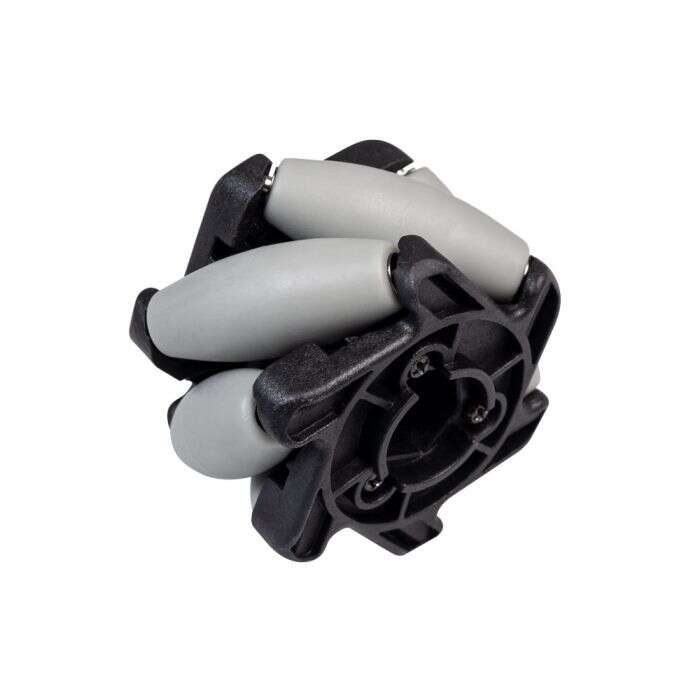
\includegraphics[scale=0.35]{Figures/mecanum1.jpg} 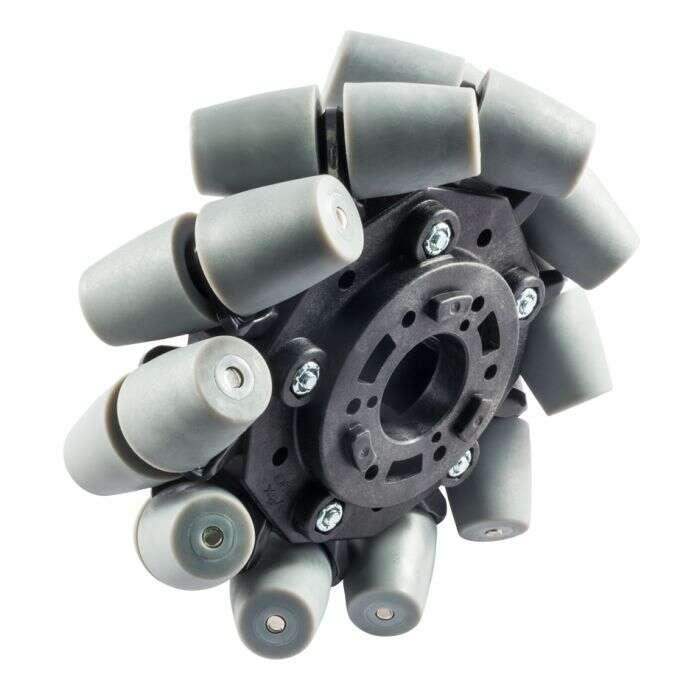
\includegraphics[scale=0.35]{Figures/mecanum2.jpg} 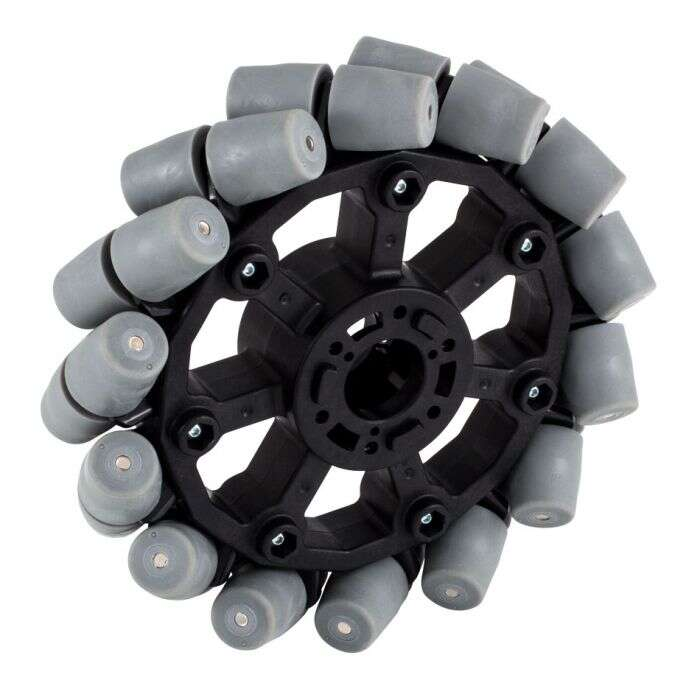
\includegraphics[scale=0.35]{Figures/mecanum3.jpg}\centering
\caption[Different variations of mecanum wheels] {Different variations of mecanum wheels \cite{diegel_improved_nodate}.}
\label{fig:differentvariationsofmecanumwheels}
\end{figure}

In the development of mecanum and other omnidirectional wheels \cite{kim_design_2001, paromtchik_practical_1994}, undesirable vibrations are frequently present in the motion due to a large number of small rollers on the wheel's periphery.

\subsection{Omnidirectional and Holonomic Motion}
A lot of design work on omnidirectional vehicles has been conducted over the years.
The earliest omnidirectional mobile vehicle to be proposed was based on introducing a methodology for the kinematic modelling of an omnidirectional wheeled mobile robot equipped with four omnidirectional wheels which were based on passive rollers arranged in an overlapping way \cite{javier_moreno_design_2016}. These wheels were positioned in pairs on the same axle but with opposite orientations. Another proposal by Wada and Mori \cite{wada_holonomic_1996} presented a new type of holonomic mobile robot which was equipped with steerable and coordinated driving wheels using conventional tires to provide an omnidirectional capability by actuating the wheels axis and a steering axis independently. In another paper by Javier Moreno, Eduard Clotet, and others design \cite{javier_moreno_design_2016} validate a three-wheel holonomic motion system for an assistant personal robot. The paper analyses the kinematics of the motion system and validates the estimation of the trajectory by comparing the displacement estimated with the internal odometry of the motors and the displacement estimated with a \ac{SLAM} procedure based on \ac{LIDAR} information . 

{\sectionbreak}
\section{Remote Control Strategies}
The remote-controlled system employs a monitor and a control device. The operator controls the remote-controlled robot with the control device while keeping an eye on the monitor, which displays visual data from the visual sensors. Expert operators who understand and are capable of training the remote-controlled robot are required to operate flexibly. Thus, operating a remote-controlled robot is difficult and may result in operational errors. This is because using a monitor that only displays visual information makes it difficult for the operator to understand real-world environmental situations. As a result, numerous stages of training are required for the operator to recognise the surroundings from visual information for expert operation \cite{masaki_remote-controlled_2022}.

Methods for improving the operability of the remote-controlled robot in terms of the mechanical design of the control device and the operation assist control method have been reported. Wireless control strategy advanced multioperability of robots \cite{almali_wireless_2015} but they are just a network to which control strategies connect to. This study proposes a remote-controlled method with an \ac{API} to improve the diversity of remote control applications. 

By combining human intuitions with the robot's motor capabilities, a motion-based control interface enables flexible robot operations in hazardous environments. It is more difficult to design a motion interface for non-humanoid robots, such as quadrupeds or hexapods, because their motions are governed by different dynamics and control techniques.
\begin{enumerate}
    \item Supervised Learning
    \par
    They employ supervised learning and post-processing techniques to convert the acquired human motion into an equivalent robot motion with appropriate semantics. They then combine motion imitation with curriculum learning to develop a control policy capable of monitoring a re-targeted reference. The authors train a group of experts to improve the performance of motion re-targeting and motion imitation. They demonstrate how the new system can perform a variety of motor activities on quadrupeds, including standing, sitting, tilting, manipulating, walking, and turning. In addition, they conduct research to determine how each component affects performance.
    \item Human Motion Control
    \par
    Human motion control allows human movements to control the robot body directly. Motion control systems relieve the human operator of the need to use traditional control devices (such as joysticks and keyboards), allowing the operator to communicate their intentions to the robot controller more effectively. As a result, human posture-based control has received a lot of attention in robotics.
\end{enumerate}

\section{Gap Analysis}
Huge leaps have been made in the development of mobile vehicles or robots with holonomic and omnidirectional motion.
Mecanum wheels have taken center stage, and the use of rollers attached to a conventional wheel has found great applications in small-scale robots and mobile platforms.
However, these wheels cannot be applied to certain applications that involve heavy payloads or rough terrains, such as moving objects in warehouses or factory floors.
Castors are predominantly used in these areas, but it involves manual control.
This process can be automated by adding motors to castors for directional control and adding the concept of remote control. Furthermore, most automated platforms have a fixed mode of control and lack the implementation of \ac{API}s embedded in their control, which necessitates this research.
  \clearpage
  \lhead{Chapter 3. Methodology}
    \chapter{Methodology}
% \newcommand{\sectionbreak}{\clearpage}
In this section, the design considerations are discussed. A detailed description of how the mobile platform will be actualized is also given. The purpose of the design process was to develop a prototype mobile platform based on caster technology. The design is a representative prototype, tailored based on $10kg$ caster wheels, which means a maximum load of 40kg would be considered for a four-wheel application. This load determines the motor and power transmission system to be applied. 


\section{Initial Considerations}
Since this is a prototype we wanted to achieve some basic minimum requirements for the robot like:
\begin{enumerate}[i.]
    \item A total payload weight of $40 kg$
    \item An average vehicle velocity of approximately $0.5m/s$ adjusted from the speed of an average human being walking of $1.3 m/s$ 
    \item An operating time of 1hr
    \item The mobile platform should not be too big and too small, the size of an average delivery box would be ideal. This is should be less than $45cm$ in length, width, and height 
    \item A mobile application to remotely control the vehicle
    \item 4 drive motors like normal electric vehicles
    \item The vehicle should accommodate a maximum incline of 5$^{\circ}$ since testing  will be conducted on a flat surface.
    \item Desired acceleration of $0.25 m/s^2$
\end{enumerate}

\section{Platform Design}
The following design considerations were made in the process of developing the physical structure of the mobile platform:
\begin{enumerate}[i.]
    \item Total load
    \item Material selection
    \item Ease of assembly and disassembly
    \item Weight of the platform
    \item Aesthetics
    \item Aerodynamics
\end{enumerate}
The mobile platform had to be lightweight and simultaneously have the ability to resist bending and compressive stresses. Table \ref{table:materialproperties} below shows the different properties of the various metals that were considered. Aluminium has the lowest mass per cubic meter and has a relatively high yield and tensile strength. It was, therefore, determined to be the best material for the platform.

\begin{table}[H]
  \begin{center}
      \leavevmode
      \hangcaption[Different Material Properties]{Different Material Properties\cite{noauthor_metal_nodate}}
     \begin{tabular}{| m{3cm} | m{2cm} | m{2cm} | m{2cm} | m{3cm} |}\hline
      Types of Metals & Tensile Strength (PSI) & Yield Strength (PSI) & Hardness Rockwell (B-Scale) & Density (\(kg/m^3\)) \\
      \hline
         Stainless steel   & 90000    & 40000 & 88 & 8000\\
         \hline
         Aluminium 6061 & 45000 & 40000 & 60 & 2720\\
         \hline
         Steel A36   & 58-80000 & 36000  & - & 7800  \\
         \hline
         Titanium & 63000 & 37000 & 80 & 4500 \\
         \hline
         Copper & 32000 & 28000 & 10 & 8940 \\
    \hline
    \end{tabular}

    \label{table:materialproperties}
  \end{center}
\end{table}

The platform design as modeled on the AutoDesk Inventor 3-D modeling software is as shown by figure \ref{fig:newfrontdwg}, figure \ref{fig:newsidedwg} and figure \ref{fig:newtopdwg}:

\begin{figure}[H]
    \centering
    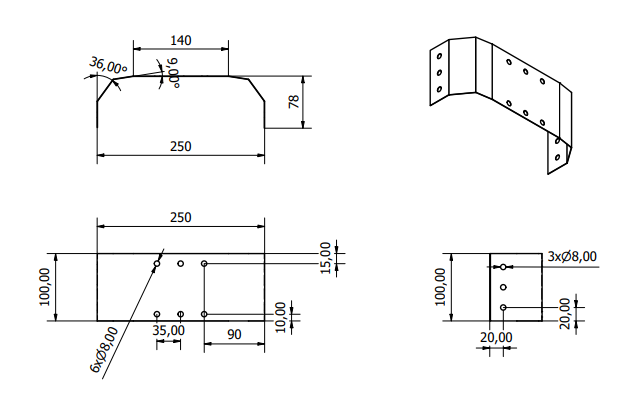
\includegraphics[scale = 0.9]{Figures/NewFrontDWG.png}
    \caption{Platform Front and Back Design}
    \label{fig:newfrontdwg}
\end{figure}

\begin{figure}[H]
    \centering
    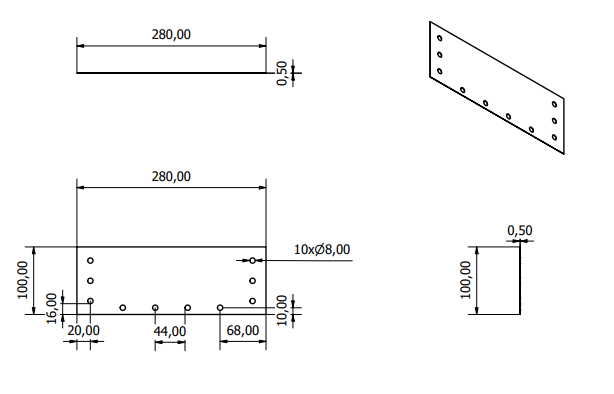
\includegraphics[scale = 0.9]{Figures/NewSideDWG.png}
    \caption{Platform Side Design}
    \label{fig:newsidedwg}
\end{figure}

\begin{figure}[H]
    \centering
    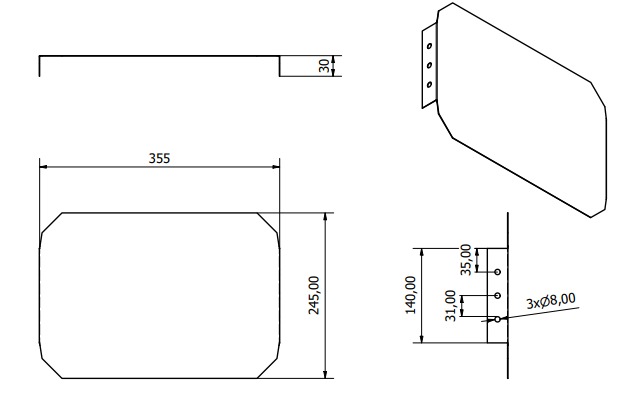
\includegraphics[scale = 0.9]{Figures/NewTopDWG.png}
    \caption{Platform Top Design}
    \label{fig:newtopdwg}
\end{figure}

Figure \ref{fig:newfrontdwg} represents the front and the back of the platform while figure \ref{fig:newsidedwg} represents the sides of the platform. Figure \ref{fig:newtopdwg} shows the design for the top of the platform. This part will hold most of the load weight. The dimensions were selected to ensure it meets a minimum size for a delivery box, that is, less than 450mm in length, width and height.

The final platform design is as shown in figure \ref{fig:platformdesign}.

\begin{figure}[H]
    \centering
    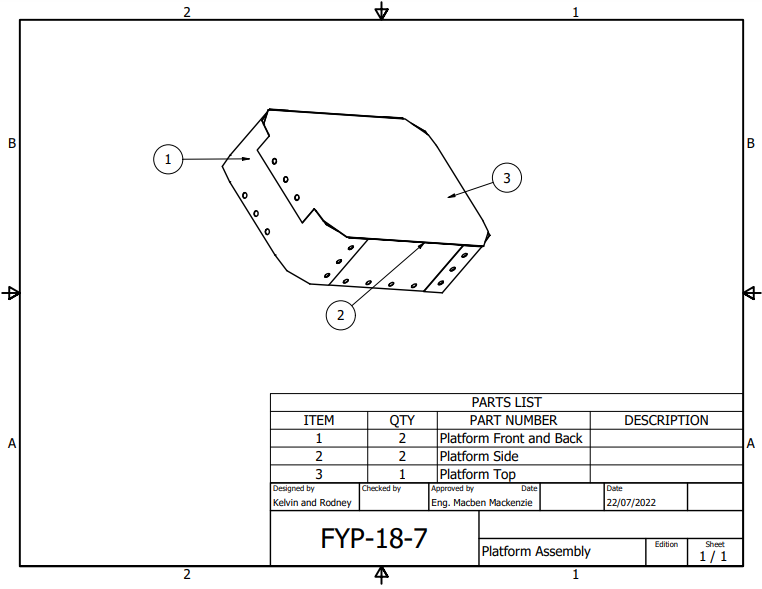
\includegraphics[scale = 0.8]{Figures/NewRedesignAssemblyParts.png}
    \caption{Platform Assembly}
    \label{fig:platformdesign}
\end{figure}

{\sectionbreak}
\section{Chassis Design}
The process of chassis design consists of:
\begin{enumerate}[i.]
    \item Load consideration
    \item Chassis type
    \item Structural analysis
\end{enumerate}

A very important consideration for chassis design is the selection of material according to the tensile strength, compressive strength, and torsional strength. The chassis carries the whole load and, therefore, the material selected needs to have high tensile strength. Table \ref{table:materialproperties} above was used to settle on steel as the preferred material. Stainless steel was considered but price was a huge factor in the design process.
\par
Other important properties are: elasticity, plasticity, hardness, toughness, dimensional stability, and durability. 
The design of the chassis has to start with consideration of load cases. The basic load cases to consider are:
\begin{enumerate}[i.]
    \item Bending case: loading in vertical plane due to the weight of components distributed along the platform frame which causes bending about the y-axis 
    \item Torsion case: vehicle body is subjected to a moment applied at the axle center lines by applying upward and downward loads at each axle. These loads result in twisting action or torsion moment about the longitudinal x-axis 
    \item Combined bending and torsion loads 
    \item Lateral loading: generated at the tire to ground contact patch. These loads are balanced by centrifugal forces 
    \item Fore and aft loading: generated when the vehicle accelerates and decelerates inertia forces 
\end{enumerate}

There are many types of chassis designs each suited to handle the load cases described above. There are ladder frames that carry all load and have good bending strength and stiffness. Other types are cruciform frames which can carry torsional loads. They are made of two straight beams and have only bending loads. The torque tube backbone (tube-frame) frame is made of a closed box section as the main backbone. Traverse beams resist lateral loads and backbone frame bending and torsion. 
\par
Considering all these properties, it was determined that a blend of cruciform frames and traverse beams would be most ideal to accommodate all forces. The developed chassis design is as shown by figure \ref{fig:newchassis}

\begin{figure}[H]
    \centering
    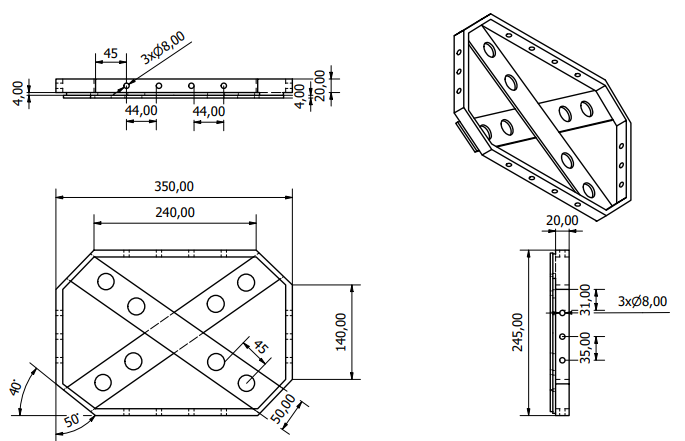
\includegraphics[scale = 0.8]{Figures/NewChassisDWG.png}
    \caption{Chassis Design}
    \label{fig:newchassis}
\end{figure}
{\sectionbreak}
\section{Wheel Frame Design}
The wheel frame was considered part of the platform and similar materials were used for the design. The frame would handle the bulk of the load and therefore a high tensile and yield strength material is required. The wheel frame would also form a housing for the motor, power transmission system, and caster wheel. These had to be considered when modeling the frame, as they have standard dimensions. Most motors have diameters ranging between $25 mm$ and $30 mm$, while their lengths range from $40 mm$ to $70 mm$. The motor selected had a diameter of 25mm and a total length of $45 mm$. The selection criteria for the motor are described in another section of this report. The power transmission system that was selected  was a belt drive with a pulley diameter of $16 mm$. The caster wheel has a standard diameter of $50  mm$.

It was therefore determined that the dimensions of the frame would be a height of $90 mm$, $50 mm$ length, and $50 mm$ width as in Figure \ref{fig:newframe}.

\begin{figure}[H]
    \centering
    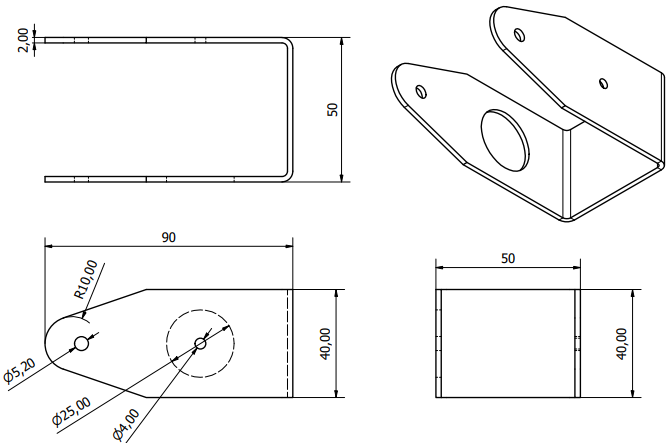
\includegraphics[scale =0.8]{Figures/NewFrameDWG.png}
    \caption{Wheel Frame Design}
    \label{fig:newframe}
\end{figure}

\begin{figure}[H]
    \centering
    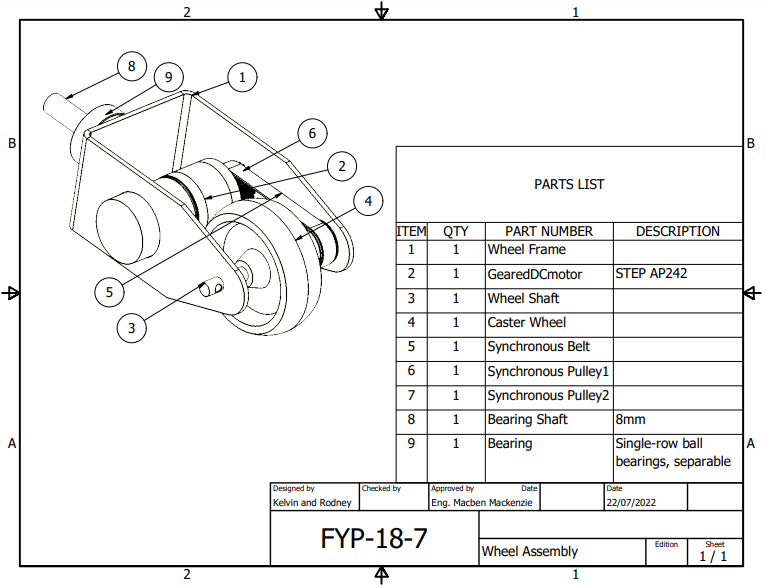
\includegraphics[scale = 0.8]{Figures/WheelAssembly.png}
    \caption{Wheel Assembly}
    \label{fig:wheelassembly}
\end{figure}

{\sectionbreak}
The final wheel frames on chassis assembly is as shown in figure \ref{fig:chassiswheel}
\begin{figure}[H]
    \centering
    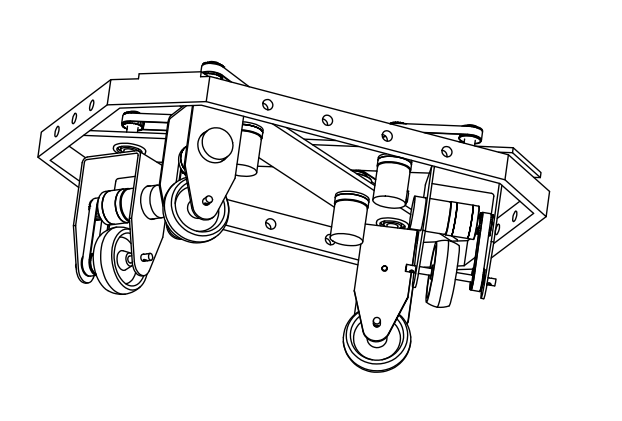
\includegraphics[scale = 0.8]{Figures/NewFinalAssemblyDWG.png}
    \caption{Wheel Frame on Chassis Design}
    \label{fig:chassiswheel}
\end{figure}

\section{Power Transmission}
The purpose of the design is to show that applying a certain amount of power to a castor wheel can do useful work and move a load, regardless of the weight. The necessary power will come from a \ac{DC} motor shaft and a power transmission system will be required to transmit power to the wheel shaft. After considering several power transmission systems, including gear drives, chain drives, and belt drives, it was determined that the latter would be most ideal for the following reasons \cite{khurmi_textbook_2005}:
\begin{enumerate}[i.]
    \item There would be a center distance between the motor and wheel shafts, a distance that would require several gears to fill making the design bulky. This eliminates gears as a means of transmission
    \item  The design does not require speed reduction which eliminates gear drives
    \item Belt drives require less maintenance than chain drives, for example, lubrication
    \item Belt drives are lighter than chain drives and gear drives, and given that the weight of the platform is one of the main design considerations, belt drives were the more preferred choice
\end{enumerate}

\subsection{Selection of a Belt Drive}
The following factors were considered when selecting a belt drive:
\begin{enumerate}[i.]
    \item The speed of the driving and driven shafts
    \item Speed reduction ratio
    \item Power to be transmitted
    \item Center distance between shafts
    \item Positive drive requirements
    \item Wheel frame dimensions
\end{enumerate}

An open belt drive is a more preferred choice than a cross belt drive due to the significantly shorter belt length. Furthermore, the belt will be made out of rubber as the material has a high load-carrying capacity compared to other belt materials. Rubber also has a long service life. The pulley material, in this case, is cast iron, and therefore the coefficient of friction between the two materials is 0.32 \cite{noauthor_pulley_nodate}.

\subsection{Speed of the driving and driven shafts}
This was going to be a low-speed application of DC motors on castor wheels which eliminated the need for any form of speed reduction. The speed reduction ratio (also the velocity ratio) is one which means that both pulleys have the same diameter. 

Velocity ratio:
%\ref{eq:3}:
\begin{equation}
\label{eq:3}
    \frac{N_2}{N_1} = \left(\frac{d_1}{d_2}\right)
\end{equation}

where: 
\begin{itemize}
\item \(d_1\)  is the diameter of the driver pulley
\item \(d_2\)  is the diameter of the driven pulley
\item \(N_1\)  is the speed of the driver pulley in rpm
\item \(N_2\)  is the speed of the driven pulley in rpm
\end{itemize}

Given that the the velocity ratio is equal to 1, \(N_1\) = \(N_2\) and \(d_1\) = \(d_2\)

\subsection{Center Distance between shafts}
This parameter determines the length of the belt. 

\begin{figure}[H]
    \centering
    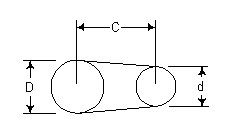
\includegraphics{Figures/NewPulley.png}
    \caption[Center distance]{Center distance\cite{noauthor_pulley_nodate}}
    \label{fig:centerdistance}
\end{figure}

The center distance is dependent on the diameters of the motor and the wheel. To make the wheel assembly design more compact, the center distance was determined to be $45mm$. The diameter of the pulleys had to be determined based on bore diameter. The bore diameter is consequently dependent on the standard wheel and motor shafts diameter. These diameters are both $5mm$ and the industry-standard outside diameter for a pulley with a 5mm bore diameter ranges from $9.68mm$ to $37.69mm$. The industry standard is 2GT synchronous pulleys and as such was used to select pulley dimensions. Again, to make the wheel assembly design more compact, an outside diameter of $16mm$ was selected for the pulley design. 
\par
Length of belt:
\begin{equation} \label{eu_eqn}
L = \frac{\pi}{2}(d_1 + d_2) + 2C + \frac{(d_1 + d_2)^2}{4C}
\end{equation}

where: 
\begin{itemize}
\item L is the total length of the belt
\item \(d_1\)  is the diameter of the driver pulley
\item \(d_2\)  is the diameter of the driven pulley
\item C is   is the center distance of the shaft
\end{itemize}

Based on the parameters established above, the total length of the belt is: 
Length of belt:
\begin{equation} \label{eu_eqn}
    \begin{aligned}
        L &= \frac{\pi}{2}(16 + 16) + 2*45 + \frac{(16 + 16)^2}{4*45}\\
        L& = 146
    \end{aligned}
\end{equation}

\subsection{Arc of Contact}

The angle of contact between the belt and pulleys as shown in Figure \ref{fig:centerdistance} is given by:
\begin{equation} \label{eqn4}
    \begin{aligned}
        &\theta_{\mathrm{d}}=\pi-2 \sin ^{-1} \frac{D-d}{2 C} \\
        &\theta_{\mathrm{D}}=\pi+2 \sin ^{-1} \frac{D-d}{2 C}
    \end{aligned}
\end{equation}


Since the pulleys have an equal diameter, the angle of contact of the belt on both pulleys is 90$^{\circ}$  or 1.57 radians.

\subsection{Power Transmitted}
The driving pulley pulls the belt from one side and delivers it to the other side. It is thus obvious that power is required. Power transmitted by a belt drive:
\begin{equation}
    Power = (T_1 + T_2)v
\end{equation}

where:
\begin{itemize}
    \item \(T_1\) is the belt tension in the tight size (N)
    \item \(T_2\) is the belt tension in the slack side (N)
    v is the belt speed. Maximum drive speed is 0.5\(m/s^2\)
\end{itemize}

Assuming that the friction is uniform throughout the arc of contact and ignoring centrifugal effects, the ratio of the tensions in the belts can be modeled by Eytlewein’s formula:
\begin{equation}
    \frac{T_1}{T_2} = e^{\mu \theta}
\end{equation}

where:
\begin{itemize}
    \item \(\theta\) is the angle of contact
    \item \(\mu\) is the coefficient of friction
\end{itemize}

The maximum allowable tension, \(T_{1,max}\), on the tight side of a belt depends on the allowable stress, \(\alpha_{max}\), of the belt material in this case rubber. 
\begin{equation}
    T_{1, max} = \alpha_{max}A
\end{equation}

where:
\begin{itemize}
    \item A is the cross-sectional area of the belt, i.e., \begin{equation}
        A = bt
    \end{equation}
    \item b is the belt width
    \item t is the belt thickness
\end{itemize}

For standard 2GT synchronous pulleys, the maximum tooth width is 11mm and maximum thickness is 1.8mm.
The maximum allowable stress for rubber is 5MPa.
\par
Therefore:
\begin{equation}
    \begin{aligned}
         T_{1,max}& =5*10^6*\frac{11}{1000}*\frac{1.8}{1000}\\
         & = 99N
    \end{aligned}
\end{equation}
Given that:

\begin{equation}
    \begin{aligned}
       \frac{T_1}{T_2}&= e^{\mu\theta},
        and\  
        T_1 = 99N,   \mu =0.32,  \theta= 1.57 radians\\
        T_2 &= 61.81N
    \end{aligned}
\end{equation}

Power transmitted by the belt drive:
\begin{equation}
    \begin{aligned}
        P &= (T_1 + T_2)v \\
        P &= (T_1 + T_2)*0.5\\
        P &= 80.4W
    \end{aligned}
\end{equation}
Torque transmitted by the belt drive:
\begin{equation}
    \begin{aligned}
        T &= (T_1 + T_2)r\\
        T &= (T_1 + T_2)\frac{8}{1000}\\
        T &= 1.28Nm
    \end{aligned}
\end{equation}

{\sectionbreak}
\subsection{Bearing Selection}
Ball bearings have standardized dimensions based on an international basis. The bearings are designated by a number. In general, the number consists of at least three digits. Additional digits or letters are used to indicate special features e.g. deep groove, filling notch, etc. The last three digits give the series and the bore of the bearing. The last two digits from 04 onwards, when multiplied by 5, give the bore diameter in millimeters.
Table \ref{table:bearingtable} shows the principal dimensions for radial ball bearings\cite{khurmi_textbook_2005}.

\begin{table}[h]
  \begin{center}
    \leavevmode
    \hangcaption[Comparison between different bearings]{Comparison between different bearings}
    \begin{tabular}{|c|c|c|c|}\hline
    Bearing No. & Bore (mm) & Outside Diameter (mm) & Width (mm) \\\hline
    200
    300 & 10 & 30
    35 & 9
    11 \\\hline
    201
    301 & 12 & 32
    37 & 10
    12 \\\hline
    202
    302 & 15 & 35
    42 & 11
    13 \\\hline
    203
    303
    403 & 17 & 40
    47
    62 & 12
    14
    17 \\\hline
    204
    304
    404 & 20 & 47
    52
    72 & 14
    14
    19 \\\hline
    205
    305
    405 & 25 & 52
    62
    80 & 15
    17
    21 \\\hline
    .
    .
    . & .
    .
    . & .
    .
    . & .
    .
    . \\\hline
    217
    317
    417 & 85 & 150
    180
    210 & 28
    41
    52 \\\hline
    218
    318
    418 & 90 & 160
    190
    225 & 30
    43
    54 \\\hline
    \end{tabular}
    \label{table:bearingtable}
  \end{center}
\end{table}


\par
The load carried by a rotating bearing is called a dynamic load. In order to select the most suitable ball bearing, the basic dynamic radial load is calculated and then multiplied by the service factor (k) to get the design basic dynamic radial load capacity. 
The approximate service life of a ball bearing is based on the fundamental equation\cite{khurmi_textbook_2005}:
\begin{equation}
    L= \frac{c}{w}^k * 10^6 revolutions
\end{equation}
or
\begin{equation}
    L = W * \frac{L}{10^6}^{\frac{1}{k}}
\end{equation}
where:
\begin{itemize}
    \item L = rating life
    \item C = basic dynamic load rating
    \item W = equivalent dynamic load
    \item k = 3, for ball bearings and \(\frac{10}{3}\) for roller bearings
\end{itemize}

\par
The relationship between the life in revolutions (L) and the life in working hours (LH) is given by L =60N.\(L_H\) revolutions  where N is the speed in r.p.m.
After finding the design basic dynamic radial load capacity, the selection of bearing is made from the catalog of a manufacturer. These load capacities are also standardized for international application.

\par
Based on these standard dimensions and load capacities, and considering that the design defines a light load application, the bearing selected lies between class 201-204. The specific bore diameter rating depends on the availability of the bearing in the market, and a 12mm bore diameter bearing would be easier to find in the market. 

\begin{figure}[H]
    \centering
    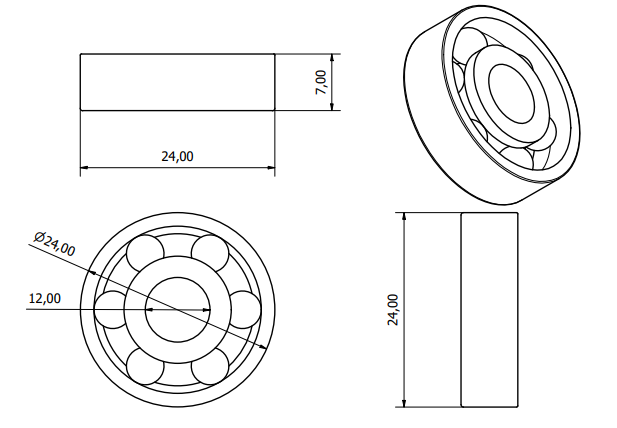
\includegraphics[scale= 0.8]{Figures/BearingDWG.png}
    \caption{Bearing Design}
    \label{fig:bearing}
\end{figure}

{\sectionbreak}
\section{Joining Methods}
The design described in this paper has several parts that require to be joined together. These parts are made of sheet metal and several types of joints were considered, including:

\begin{enumerate}[i]
    \item Screw joints
    \item Rivet joints
    \item Welded joints
    \item Folding/Tab joints
    \item Adhesive joints
\end{enumerate}

The screw joint is a type of a temporary joint. Screws, bolts, nuts, studs and standoff are used for fastening sheet metal parts. Machine screws and self tapping screws are the two types of screws commonly used. Self tapping screws are a low-cost solution for a one time assembly of parts. Machine screws, on the other hand, are suitable for applications where multiple assemblies and disassembly are required \cite{admin_how_2018}. It was therefore determined to be the most suitable joining technique for the design. Screws are additionally the best choice for softer materials such as aluminium.
\par
The rivet joint is a simple, convenient and fast joining technique. However, it requires applications where disassembly is not an option since it is a permanent joining technique. It was therefore determined to be unsuitable for this particular design.
\par
Welding is also a permanent joining technique. Several techniques are used for joining sheet metal parts including arc welding, gas welding and tungsten inert welding. Several considerations need to be made when applying this method, such as:
\begin{enumerate}[i]
    \item Sheet metal material
    \item Sheet metal thickness
    \item Final finish requirements
    \item Airtight or waterproof requirements
\end{enumerate}

The sheet metal material used in the design is aluminium, which has a low melting point of 660$^{\circ}$ \cite{noauthor_aluminium_nodate}  that would be unsuitable when joining using an arc weld. The sheets would melt before a joint was formed. The parts in the design will have a  metal thickness of $2mm$, which is unsuitable for welding since welding thin metals can cause warping and burn-through. Welded joints have a poor surface finish, and since aesthetics are a main consideration in the design process, welding would be ill-suited for joining the parts.
\par
Folding or bending tabs are an economical way of making permanent sheet metal joints. They are accomplished using sheet metal bending machines, therefore requires very little hardware setup. Tab joints are suitable for soft material such as aluminium. Adhesive joints are a type of permanent joint where adhesives are placed between the part surfaces and then pressure is applied. To disassemble the parts, chemicals can be applied which is not economical especially for small applications. 
\par
Having considered several joining techniques, screws or fasteners were resolved to be most suitable for the design and ultimately fabrication of the mobile platform. 

\section{Motor Sizing}

The motor is responsible for supplying the drive to the transmission system responsible for the movement of the robot. There are numerous motor types that can be used in robotic applications. Each type of motor serves a distinct purpose. The motors help the robot move and act as actuators in the mechanical design of the robot. Since this is a mobile robot with a small payload size, \ac{AC} motors are ruled out. The remaining \ac{DC} motors used for locomotion are:
\begin{enumerate}[i.]
    \item Brushed \ac{DC} motors use brushes to conduct current between the source and the armature. There are several types of brushed \ac{DC} motors, but permanent magnet \ac{DC} motors are used in robotics. These motors have a high torque-to-inertia ratio. Brush \ac{DC} motors are capable of producing torque three to four times greater than their rated torque.The brush \ac{DC} motors have two terminals. When a voltage is applied across the two terminals, a proportional speed is an output to the brush \ac{DC} motor's shaft.

    \item Brushless \ac{DC} motors are built similarly to brushed \ac{DC} motors, but they are controlled by closed-loop controllers and require inverters or \ac{SMPS} for power. Permanent magnets rotate a fixed armature in these motors. Unlike Brush \ac{DC} motors, they have a closed-loop electronic controller instead of a commutator assembly. These motors are typically used in industrial robotics where precise motion and positioning control are required. These motors, however, are quite expensive and involve complex construction and electronics.

    \item Geared \ac{DC} motors are a more advanced version of brush \ac{DC} motors. A gear assembly is attached to the motor. The motor's speed is reduced as the torque increases thanks to the gear assembly. The speed of the \ac{DC} motor can be reduced while increasing torque by using the proper combination of gears to the motor. This ensures that the motor rotates steadily and that it can be stopped or changed the speed in a controlled manner. \ac{DC} motors operate within a specific voltage range, and the higher the input voltage, the higher the \ac{RPM}.
\end{enumerate}

When selecting the right motor to use in this application, a motor that could be able to provide us with high torque of approximately $1 Nm$ to be able to carry a payload of $40 kg$ at a low speed is considered. The operating voltage as it has a direct correlation with the power we can draw from the battery, thus influencing the capacity of our battery is also considered. Cost and availability should be top priorities. A geared \ac{DC} motor is selected as shown in Table \ref{table:comparedifferentmotrs}.

\begin{table}[ht]
  \begin{center}
    \leavevmode
    \hangcaption[Comparison between different motors]{Comparison between different motors}
    \begin{tabular}{|c|c|c|c|}\hline
    Parameters & Brushed \ac{DC} motors & Brushless \ac{DC} motors & Geared \ac{DC} motors \\\hline
    Speed & Fast & High & Low \\\hline
    Torque & Low & Low & High \\\hline
    Cost & Inexpensive & Expensive & Inexpensive \\\hline
    Availability & Available & Available & Available \\\hline
    Operating Voltage & $6 V$ - $12 V$ & $12 V$ & $6 V$ - $12 V$ \\\hline
    Lifetime & Short & Long & Short \\\hline
    Efficiency & Low & High & Low \\\hline
    Noise & High & Low & Low \\\hline
    \end{tabular}
    \label{table:comparedifferentmotrs}
  \end{center}
\end{table}

Some of the design considerations that are considered in the process of selecting the specific \ac{DC} motors are:
\begin{enumerate}[i.]
    \item  Nominal Voltage. The higher the voltage, the better as less current will be needed to supply the electrical power to the motors. A $6 V$ motor will draw twice as much current as a $12 V$ motor for the same application 
    \item No Load \ac{RPM} and full load \ac{RPM}
    \item Stall current and Stall torque - The system ought to be designed to never allow the motor to come anywhere near this point, This can done by ensuring the motor operated at at least 30\% of the stall torque.
    \item Gear down - This helps to achieve the required torque at the output of the shaft and allows the transmission unit to run at a gear ratio of 1:1. The output speed is reduced to a manageable level while the torque is increased.
    \item Rotary encoders. This would be a great addition, but to find a geared \ac{DC} motor with the rotary encoder attached to it is difficult.
\end{enumerate}

The torque required by the motor is determined as follows based on Figure \ref{fig:simpletorque}:

\begin{figure}[h]
    \centering
    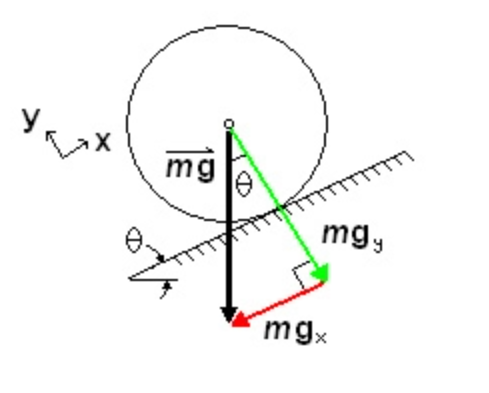
\includegraphics[scale=0.5]{Figures/simpleTorque.png}
    \caption{Simple Torque Representation On an Inclined Surface}
    \label{fig:simpletorque}
\end{figure}

From Figure \ref{fig:simpletorque} with a $5^{\circ}$ inclined surface, only one component of its weight, $mg_x$ parallel to the surface, causes the robot to move downwards. The other component, $mg_y$, is balanced by the normal force the surface exerts on the wheels. $mg_x$ is calculated as shown by Equation \ref{mgxcalculations} and $mg_y$ is calculated as shown by Equation \ref{mgycalculations}


\begin{equation} \label{mgxcalculations}
\begin{split}
mg_x & = mg * sin (\theta) \\
& = 45 * 9.81 * sin (5) \\
& = 38.4749 N 
\end{split}
\end{equation}

\begin{equation} \label{mgycalculations}
\begin{split}
mg_y & = mg * cos (\theta) \\
& = 45 * 9.81 * cos (5) \\
& = 439.7701 N
\end{split}
\end{equation}


For the robot not to slide down the incline, there must be friction between the wheel and the surface. 
The torque (T) required is given by equation \ref{torqueeqn}.

\begin{equation} \label{torqueeqn}
T = f * R
\end{equation}

To select the proper motor, we must consider the "worst-case scenario," where the robot is not only on an incline but accelerating up it.
Note now that all forces ($F$) are along the x and y axes. We balance the forces in the x-direction as shown by equation \ref{balanceforces}

\begin{equation} \label{balanceforces}
\begin{split}
F_x & = m * a  \\
& = f - m g_x \\
& = \frac{T}{R} - m g_x
\end{split}
\end{equation}

% \begin{flushleft} \label{balanceforces}

% \end{flushleft}

\begin{equation} \label{totaltorqueeqn}
T = R * M *( a + g * sin(\theta))
\end{equation}

This torque given by equation \ref{totaltorqueeqn} value represents the total torque required to accelerate the robot up an incline. However, this value must be divided by the total number ($N$) of drive wheels to obtain the torque needed for each drive motor. The final point to consider is the efficiency ($e$) of the motor, gearing, and wheel (slip). This results to the torque required by each wheel as shown by equation \ref{totaltorqueeqnwithefficiency}

\begin{equation} \label{totaltorqueeqnwithefficiency}
T = \frac{100}{e} * \frac{R * M *( a + g * sin(\theta))}{N}
\end{equation}

The value for efficiency here represents the total efficiency, as shown by equation \ref{totalefficiency}, of the system and can be estimated as follows:
\begin{itemize}
    \item Battery to Motor Controller: 90\% efficient
    \item Motor Controller to Motors: 70\% efficient
    \item Transmission to Wheels 80\% efficient
\end{itemize}
The lost energy is transferred mostly to heat and noise.

\begin{equation} \label{totalefficiency}
\begin{split}
e & = 0.9 * 0.7 * 0.8 \\
& = 50.4\% \\
\end{split}
\end{equation}

With a total efficiency of the system as $50.4\%$ torque required by each wheel is calculated as shown in equation \ref{totaltorque}.

\begin{equation} \label{totaltorque}
\begin{split}
T & = \frac{100}{50.4} * \frac{0.015 * 45  *( 0.25 + 9.81 * sin(5))}{4} \\
& = 0.37 Nm \\
\end{split}
\end{equation}

With this a motor of $12V$ $250$ \ac{RPM} \ac{DC} motor of $0.8629 N/m$ in torque can suffice for this operation. This motor can provide the required torque for this application but the Speed will be reduced to $0.3927 m/s$ as shown by equation \ref{speedmpers} which is not far off from the expected $0.5 m/s$.

\begin{equation} \label{speedRadians}
w = \frac{2 * \pi * N}{60}
\end{equation}

\begin{equation} \label{speedmpers}
\begin{split}
v & = r * w\\
& = 0.015 * \frac{2 * \pi * 250}{60} \\
& = 0.3927 m/s 
\end{split}
\end{equation}

The total power ($P$) per motor can be calculated using the following relation:

\begin{equation} \label{totalefficiency}
\begin{split}
P & = T * w\\
& = 0.37 * \frac{2 * \pi * 250}{60} \\
& = 9.6866W 
\end{split}
\end{equation}

\begin{equation} \label{totalefficiency}
\begin{split}
I & = \frac{P}{V}\\
& = \frac{9.6866 W}{12 V} \\
& = 0.8072 A
\end{split}
\end{equation}


The maximum current that id drawn from a battery is $0.4843A$ to be supplied to the motors.

Finally, the capacity ($C$) of the battery pack required can be estimated using the equation \ref{batterycap}:

\begin{equation} \label{batterycap}
\begin{split}
C & = I * t\\
& = 0.8072 * 1 \\
& = 0.8072Ah \\
& = 0.8072 * 8 \\ 
& = 3.2288 Ah \\
\end{split}
\end{equation}

With a $3.2 Ah$ battery the motors will be able to run the mobile platform for 1hr without recharging.

\section{Motor Control}

A \ac{DC} motor controller is any device that can manipulate the position, speed, or torque of a \ac{DC}-powered motor. Control of the speed and rotation of the \ac{DC} motor is critical. The speed/torque curve of \ac{DC} motors is inversely linear, meaning their torque proportionally decreases as the motor \ac{RPM} increase. This allows for easy control, as lowering the speed will increase the torque, and vice versa.

\subsection{Direction Controller: H Bridge}

A H bridge circuit is one of the simplest methods to control a \ac{DC} motor. There are four switches controlled in pairs (1 \& 4, 2 \& 3) as shown in Figure \ref{fig:directionControl}, and when either of these pairs is closed, the circuit is completed and the motor is powered. Depending on the orientation of the motor when 1 \& 4 are closed the motor move clockwise while when 2 \& 3 are closed the motor moves anticlockwise.


\begin{figure}[H]
    \centering
    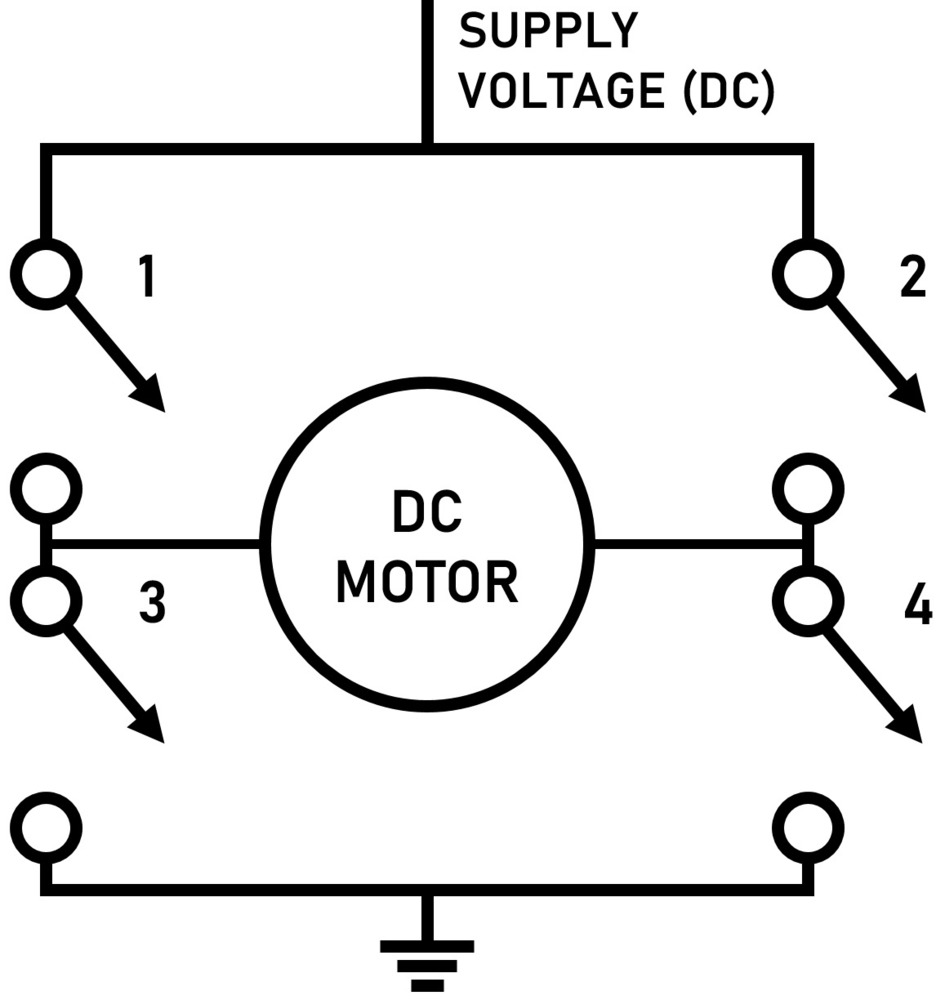
\includegraphics[scale=0.2]{Figures/DirectionControl.jpg}
    \caption[Direction Control]{Direction Control \cite{noauthor_all_nodate}}
    \label{fig:directionControl}
\end{figure}

A four-quadrant motor can thus be created by connecting certain switches, the polarities of which change to produce different effects on the motor as shown in Figure \ref{fig:4quadrantops}. This circuit essentially switches the leads of the DC motor, which will reverse its rotational direction on command. Most DC motors are slowed by simply cutting power to the motor; regenerative drives include braking capabilities, which cause deceleration by switching polarities while the motor is running. Non-regenerative drives control quadrants 1 and 3, which are considered "motoring" quadrants because the motor provides acceleration in either direction. Quadrants 2 and 4 are considered "braking" quadrants because the motor is decelerating and is used by regenerative drives. When the motor speed opposes the motor torque, the motor transforms into a generator, and its mechanical energy drives a current back to the power source (a process known as "regenerative braking"). This feature reduces energy losses and allows the power source to be recharged, effectively increasing motor efficiency.

\begin{figure}[h]
    \centering
    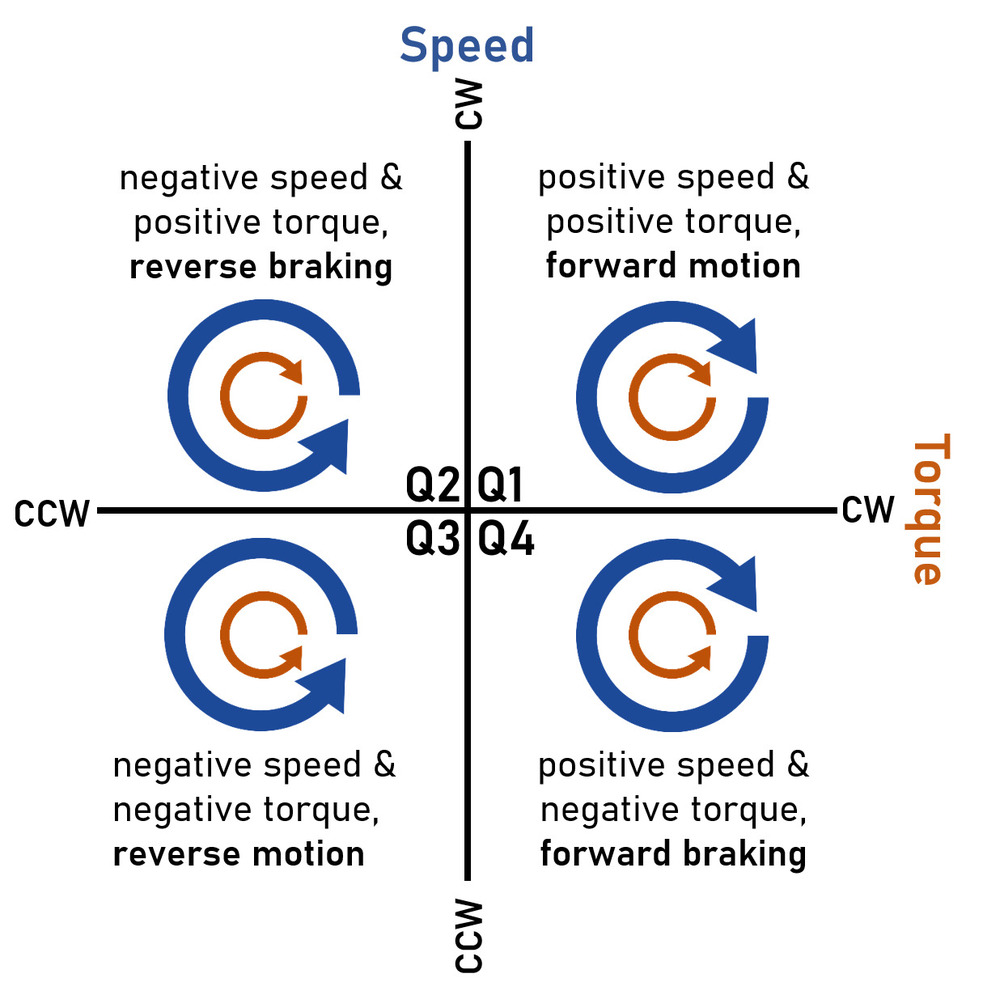
\includegraphics[scale=0.3]{Figures/4Quadrant.jpg}
    \caption[4 Quadrant Operation]{4 Quadrant Operation \cite{noauthor_all_nodate}}
    \label{fig:4quadrantops}
\end{figure}

\subsection{Speed Controller: Pulse Width Modulation (PWM)}

PWM circuits control motor speed by simulating a change in supply voltage. Adjustable speed drive controllers send periodic pulses to the motor, which, when combined with the smoothing effect of coil inductance, causes the motor to behave as if it is powered by a lower/higher voltage. The percentage of voltage reduction, or the PWM "duty cycle," will thus affect the motor's speed. PWM is simple and inexpensive to implement, and virtually Any duty cycle can be selected, allowing for almost continuous motor speed control. PWM is frequently used in conjunction with H bridges to control speed, direction, and braking.When the duty cycle is reduced to one quarter of the total time, the effective voltage is about one quarter of the total voltage.
Some of the factors that were considered when choosing a motor driver were:

\begin{enumerate}[i.]
    \item Ability to both control speed and rotations
    \item The higher the number of motor output the better
    \item The operating voltage should be inclusive of our motor voltage of 12V.
    \item The higher the efficiency the better. \ac{MOSFET} controlled drivers have a higher efficiency that \ac{BJT}.
    \item A small form factor would be better
    \item Maximum current it can supply to the motors should be approximately 1A needed generate our required torque of $0.37 N m$
\end{enumerate}
% REF 
The Satima S2 motor driver was best suited for this application. This is because it can operate our 12V motor voltage, can supply up to a maximum of 3A per channel and High-Noise-Immunity Inputs. All in all it is \ac{MOSFET} controlled making it to have a higher efficiency.

\begin{figure}[H]
    \centering
    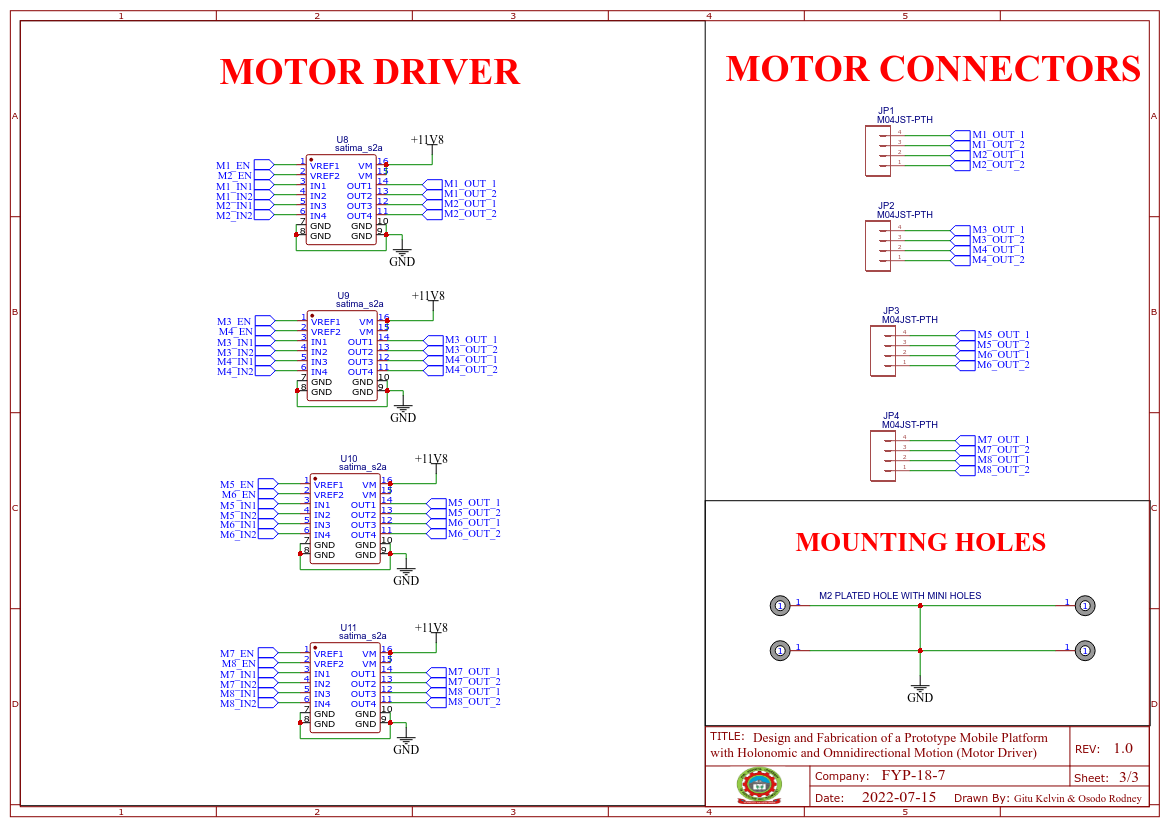
\includegraphics[scale=0.4]{Figures/MPmotorDriver.png}
    \caption{Motor Driver Schematic}
    \label{fig:motordriverschematic}
\end{figure}

Figure \ref{fig:motordriverschematic} shows the Motor Driver Part of the Mobile Platform. There are 8 motors controlled by 4 motor drivers which can be able to control 2 motors per motor driver. The Connectors are JST connectors as the are strong and reliable.
The mounting holes are connected to ground as they will be screwed on to the platform.

\section{Remote Control Clients}

\ac{API} are code snippets that allow software applications to communicate in a common language and are becoming increasingly common in today's consumer and business environments. Web APIs enable client applications to access third-party data and seamlessly integrate it wherever and whenever it is needed, providing unrivalled data processing efficiencies and cost savings.

\ac{API} offer scalability, extended Reach, 3rd party integrations, speed, simplicity and customization. As shown by figure \ref{fig:omicronplatformcontrol} the goal is to abstract the robot control using an \ac{API}. This will ensure the building of different client applications to control the robot. A hand motion control, a hardware interface, and a mobile application, a software interface, will be the applications built to control the robot.

The \ac{API} will be abstracted on the internet as a Website Application Server. This will route traffic to the mobile platform through \ac{MQTT}. The protocol is event-driven and uses the publish/subscribe (Pub/Sub) pattern to connect devices. Topics are used to communicate between the sender (Publisher, Web \ac{API}) and the receiver (Subscriber, Mobile Platform). The \ac{MQTT} broker manages the connection between them. All incoming messages are filtered by the \ac{MQTT} broker. The WiFi client will send the data to the main CPU for processing. The \ac{COAP} was not used as its support is low in hobbyist market and it is more suited for industrial applications.

Figure \ref{fig:omicronplatformcontrol} shows how the architecture will be laid out. Having different clients that can be abstracted by the Web Application increase the type of control mechanisms used to control the robot. For this, hand motion control and mobile application control will be demonstrated as examples of both hardware and software control mechanisms.

\begin{figure}[H]
    \centering
    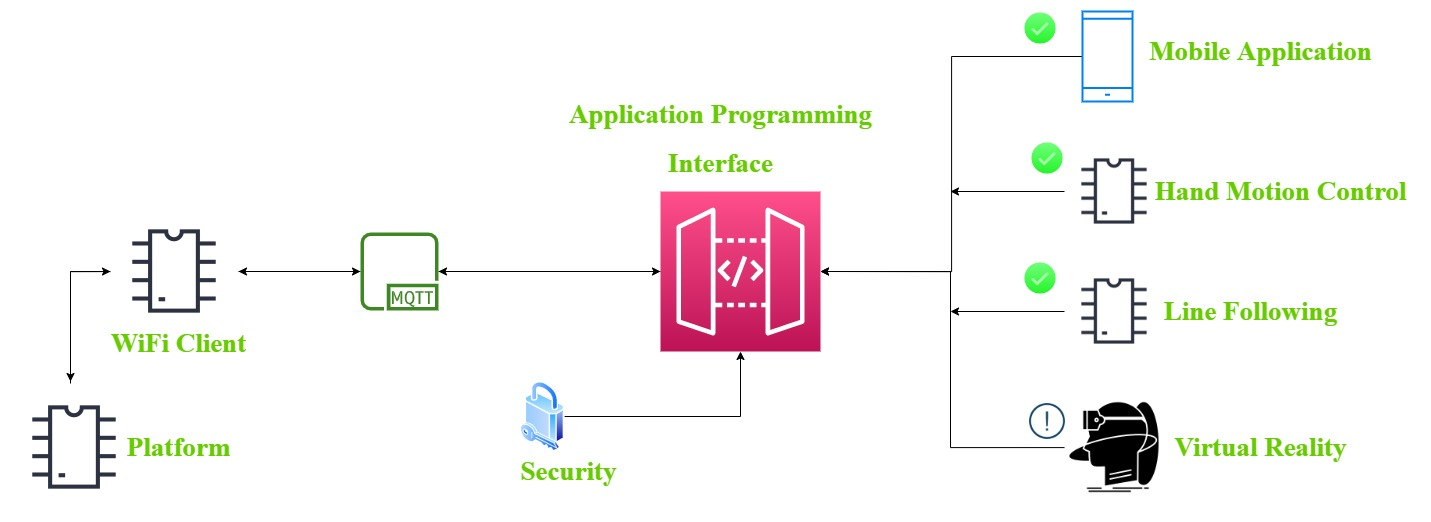
\includegraphics[scale=0.3]{Figures/omriconrobotPlatformControl.jpg}
    \caption{Mobile Platform Architecture}
    \label{fig:omicronplatformcontrol}
\end{figure}

\subsection{Hand Motion}

This is a hardware client that maps hand motion to actual commands to be sent to the mobile platform. The working of the hand motion control is demonstrated by figure \ref{fig:handmotioncontrol}. When a user emulated a recognised hand motion we will decode it to a form that the mobile platform can understand then send it to the mobile platform. We don't need to know the actual hand motions as with a fuzzy controller we are able to map any input to match the mobile platform specified motions.

The hand motion as shown by figure \ref{fig:handmotionschematic} will constitute mainly of an Inertial Measuring Sensor to detect the different hand motions. The Central Processing Unit will interpret the motions and transmit the command wireless to the mobile platform.

\begin{figure}[H]
    \centering
    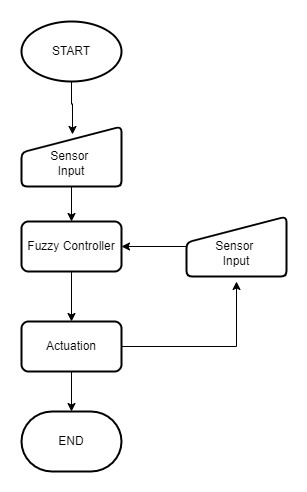
\includegraphics[scale=0.5]{Figures/linefollowing-handmotion.jpg}
    \caption{Hand Motion Control Strategy}
    \label{fig:handmotioncontrol}
\end{figure}

\begin{figure}[H]
    \centering
    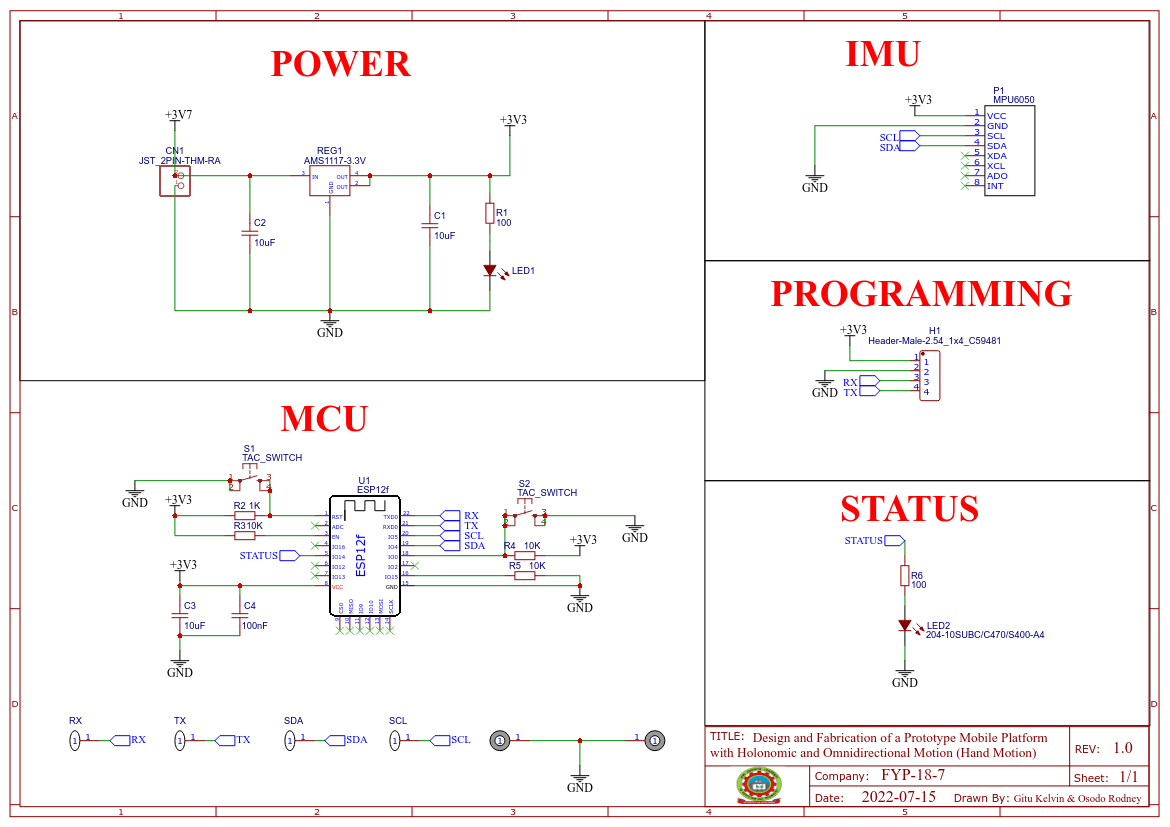
\includegraphics[scale=0.4]{Figures/HMSchematic.png}
    \caption{Hand Motion Schematic}
    \label{fig:handmotionschematic}
\end{figure}

\subsection{Mobile Application}

This is a software client that maps input from the application to actual commands to be sent to the mobile platform. For the mobile platform the best implementation is currently based on Flutter framework and Dart Language. Flutter is an open source framework by Google for building beautiful, natively compiled, multi-platform applications from a single code base. Features are created from widgets which are simple to design allowing for speedy development.
Figure \ref{fig:handmotionmobileapp} shows the process of how the mobile application will be working.

\begin{figure}[H]
    \centering
    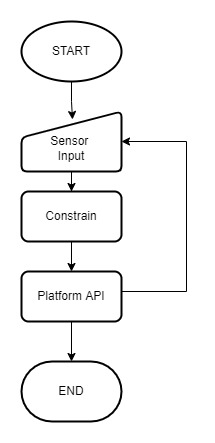
\includegraphics[scale=0.5]{Figures/linefollowing-mobileapp.jpg}
    \caption{Mobile application Strategy}
    \label{fig:handmotionmobileapp}
\end{figure}

\section{Electronics}

This is the brain of the mobile platform and is responsible in converting the user input to motor rotation and translational values. The main compute platform is responsible in controlling the motors individually to achieve holonomic control. Though automobiles have coupled mechanics to drive the wheels, we will ensure that the motors are coupled through the software for synchronised motion.

\begin{figure}[H]
    \centering
    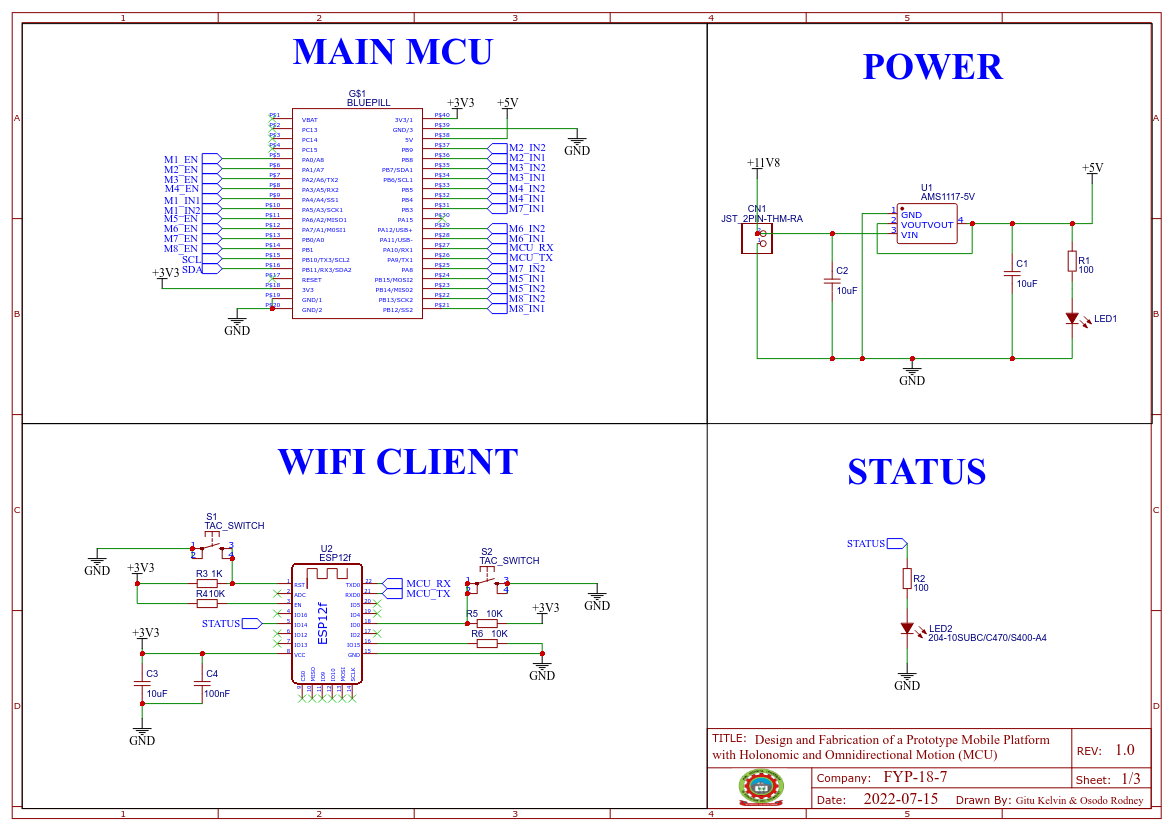
\includegraphics[scale=0.4]{Figures/MPmain.png}
    \caption{Mobile Platform Main Schematic View}
    \label{fig:mobileplatformmain}
\end{figure}


The considerations that went into selecting the microcontroller were:
\begin{enumerate}[i]
    \item It should be compatible with all auxilliary components including the motor and the inertial measuring sensor
    \item It should have on board features such as integrated Wi-Fi support and USB port
    \item It should have enough processing power to reduce latency during operations such as wireless communication.
    \item Its memory should be enough to accommodate the written program with all of its functionality.
    \item It should have the desired number of GPIO pins.
\end{enumerate} 

\par
The STM32 and Arduino microcontrollers were considered as they are the most common and prevalent in the market. The STM32 microcontroller, more specifically STM32F103C8T6 was chosen as main microcontroller unit \ac{MCU}, and the main deciding factor was the number of pins on the \ac{MCU}. It has 40 pins which would comfortably accommodate the more than 24 pins required to operate eight \ac{DC} motors.
\par
For the Wi-Fi client, the ESP-12f was chosen. This module supports the standard IEEE802.11 b/g/n protocol, a complete
TCP/IP protocol stack. It adds networking capabilities to existing devices and can be used to build separate network controllers. It is also highly cost effective compared to other modules such as ESP32.

\par
Figure \ref{fig:mobileplatformmain} also shows the circuitry for the power unit. In order to operate the mobile platform for at least an hour, a high capacity (greater than 900mAH) power source that can be recharged was the desired supply for the platform. Looking across the market, the 18650 Lithium Ion Battery 2200mAh 3.7V was selected as most suitable for the job.

\begin{figure}[H]
    \centering
    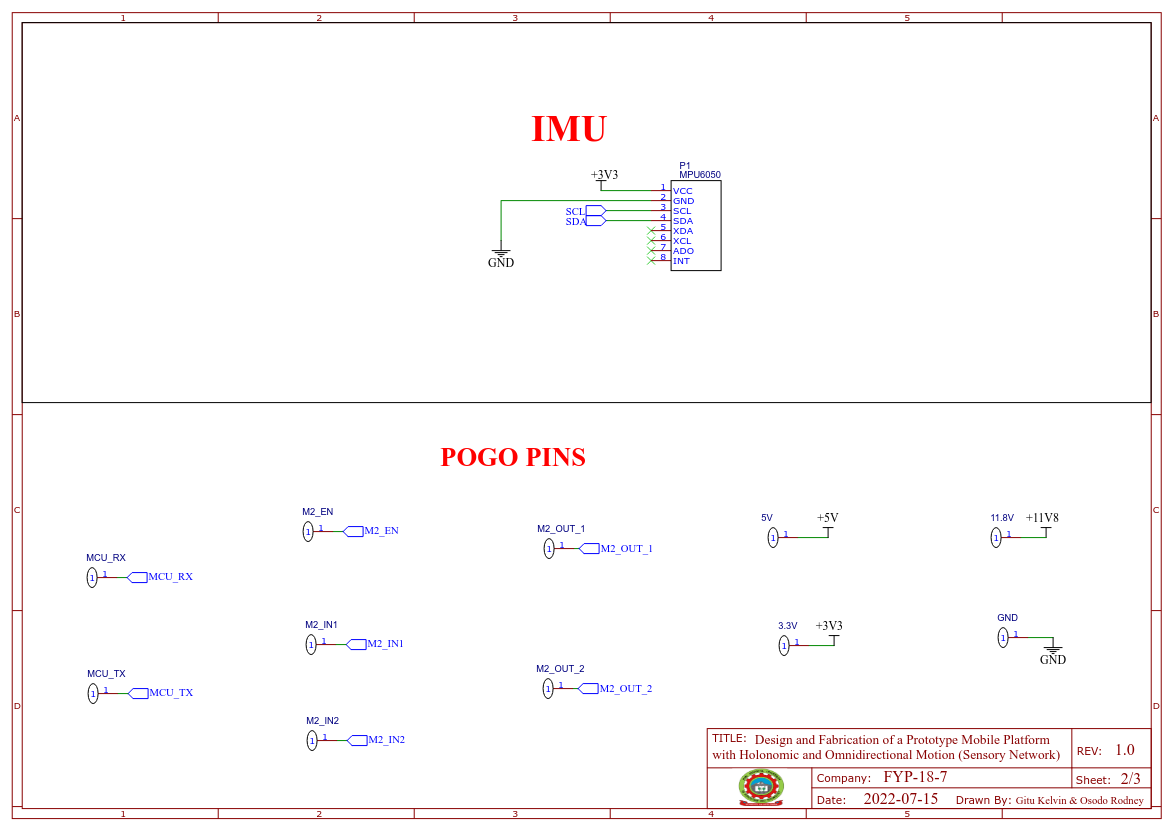
\includegraphics[scale=0.4]{Figures/MPsensory.png}
    \caption{Mobile Platform sensory schematic}
    \label{fig:mobileplatformsensory}
\end{figure}

\par
An Inertial Measurement Unit, also known as \ac{IMU}, is an electronic device that measures and reports acceleration, orientation, angular rates, and other gravitational forces. It is composed of 3 accelerometers, 3 gyroscopes, and depending on the heading requirement – 3 magnetometers. That is to say, one per axis for each of the three vehicle axes: roll, pitch, and yaw.

There are different types of \ac{IMU} sensors \cite{noauthor_imu_nodate}: the one based on FOG (Fiber Optic Gyroscope), the RLG \ac{IMU}s (Ring Laser Gyroscope), and lastly, \ac{IMU} based on MEMS technology (Micro Electro-Mechanical Systems). This technology allows lower costs and low power requirements while ensuring performance. MEMS-based systems therefore combine high performance and ultra-low power in a smaller unit.
\par
The \ac{IMU} selected for this particular application is the MPU6050 sensor module which is a complete 6-axis Motion Tracking Device. It combines 3-axis Gyroscope, 3-axis Accelerometer and Digital Motion Processor all in small package\cite{noauthor_mpu6050_nodate}. It also has additional feature of on-chip temperature sensor. 

\begin{figure}[H]
    \centering
    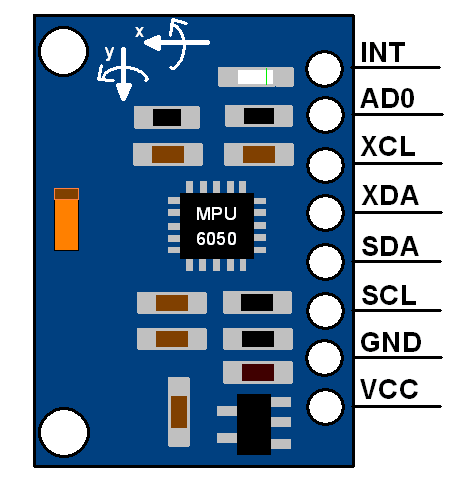
\includegraphics[scale=0.8]{Figures/MPU6050_Module.png}
    \caption{MPU6050 Sensor Module}
    \label{fig:my_label}
\end{figure}

% \section{Software Architecture}


  \clearpage
  \lhead{Chapter 4. Results and Discussion}
    \chapter{Results and Discussion}
\section{Final Design}

\begin{figure}[h]
    \centering
    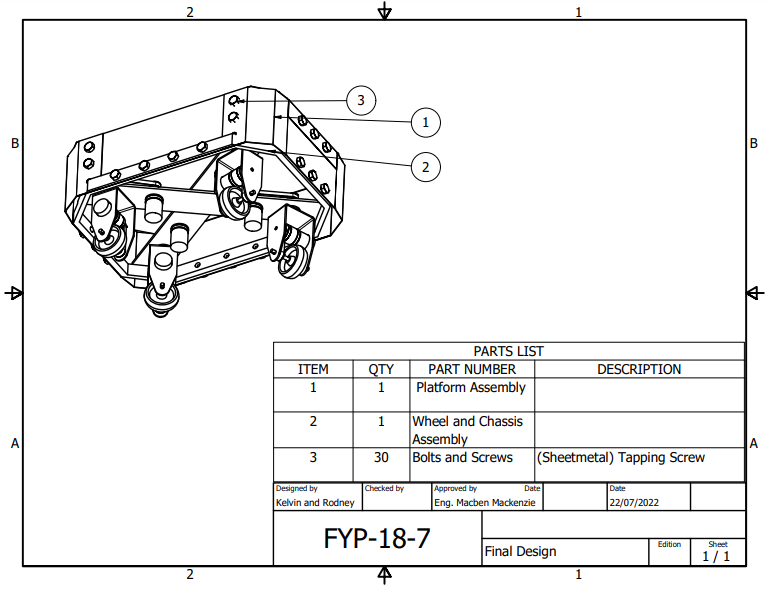
\includegraphics[scale = 0.7]{Figures/NewFinalAssemblyParts.png}
    \caption{Final Design}
    \label{fig:finalassemblyparts}
\end{figure}

\begin{figure}[h]
    \centering
    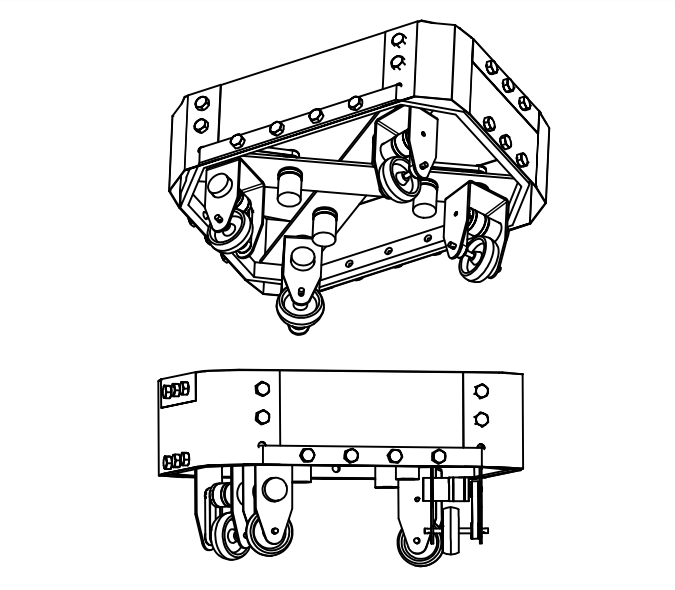
\includegraphics[scale = 0.8]{Figures/NewFinalDesignDWG.png}
    \caption{Final Assembly}
    \label{fig:finalassembly}
\end{figure}

\section{Load analysis on Platform}

\begin{figure}[H]
    \centering
    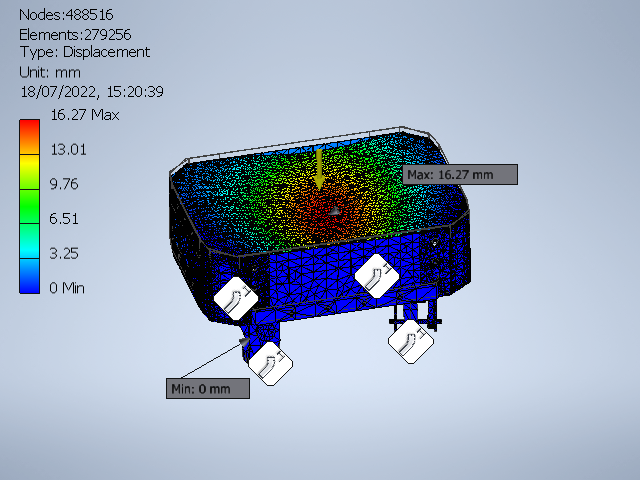
\includegraphics[scale = 0.9]{Figures/PlatformDisplacement.png}
    \caption{Displacement by Load}
    \label{fig:platformdisplacement}
\end{figure}

A force of $400N$ was applied on the platform top to simulate a practical load of $40kg$ on the platform. The results indicate a displacement of $16.27mm$ in the Z-axis at the point of application. However, since the load will be distributed evenly on the platform surface this displacement will be evenly distributed along the platform and won't be as apparent practically.
\par
This displacement will also be alleviated by adding a support shaft that rests on the chassis. The analysis also suggested a maximum safety factor of $15$ as shown on Figure \ref{fig:safetyfactor} on areas that receive little force and a safety factor of between $3$ and $6$ for the top of the platform. This allows a force up to six times the base force of $400N$ before the platform fails.

\begin{figure}[H]
    \centering
    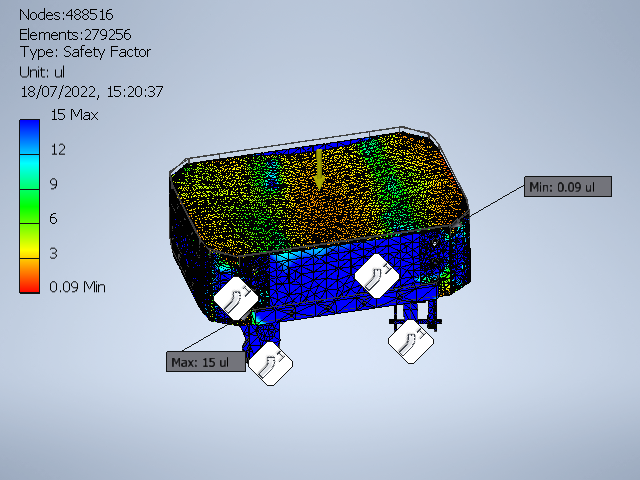
\includegraphics[scale = 0.9]{Figures/safety_factor.png}
    \caption{Safety Factor}
    \label{fig:safetyfactor}
\end{figure}

\section{Load analysis on Chassis}

\begin{figure}[H]
    \centering
    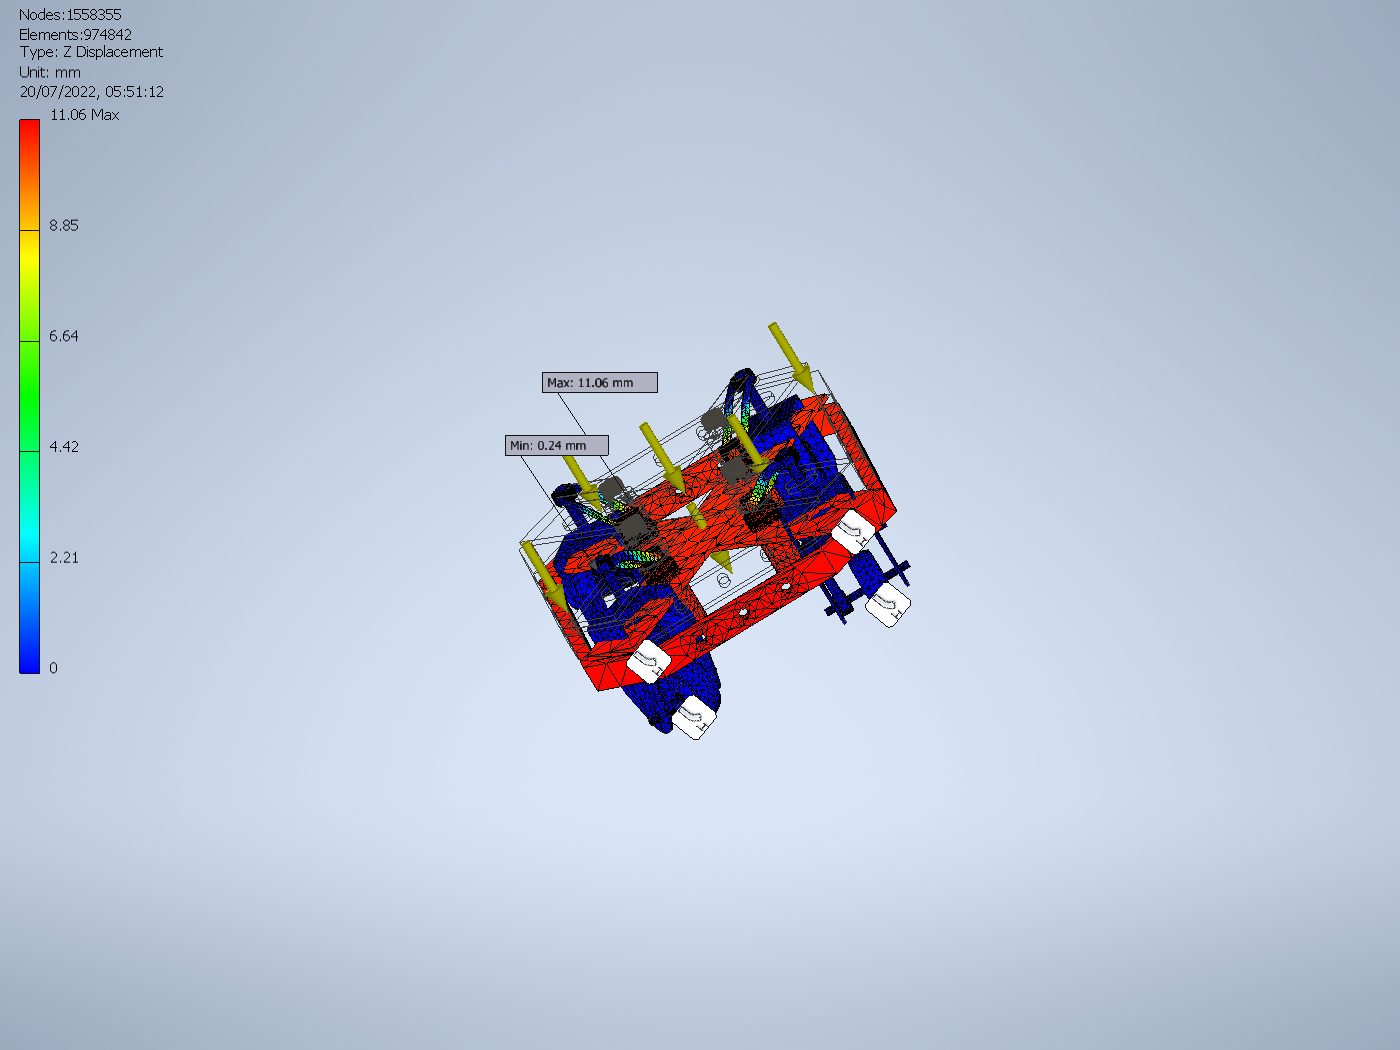
\includegraphics[scale = 0.4]{Figures/ChassisDisplacement.png}
    \caption{Displacement of Chassis by load}
    \label{fig:chassisdisplacement}
\end{figure}
\par
The analysis results showed that the chassis can handle the maximum load desired, albeit a displacement of $11.06mm$. This displacement is concentrated at the centre of application of the force, but since the force will be evenly distributed across all chassis faces, the expectation is that the displacement will be minimum. The chassis should comfortably carry the weight.

% \section{Torque analysis on Wheel Frame}

% \begin{figure}[H]
%     \centering
%     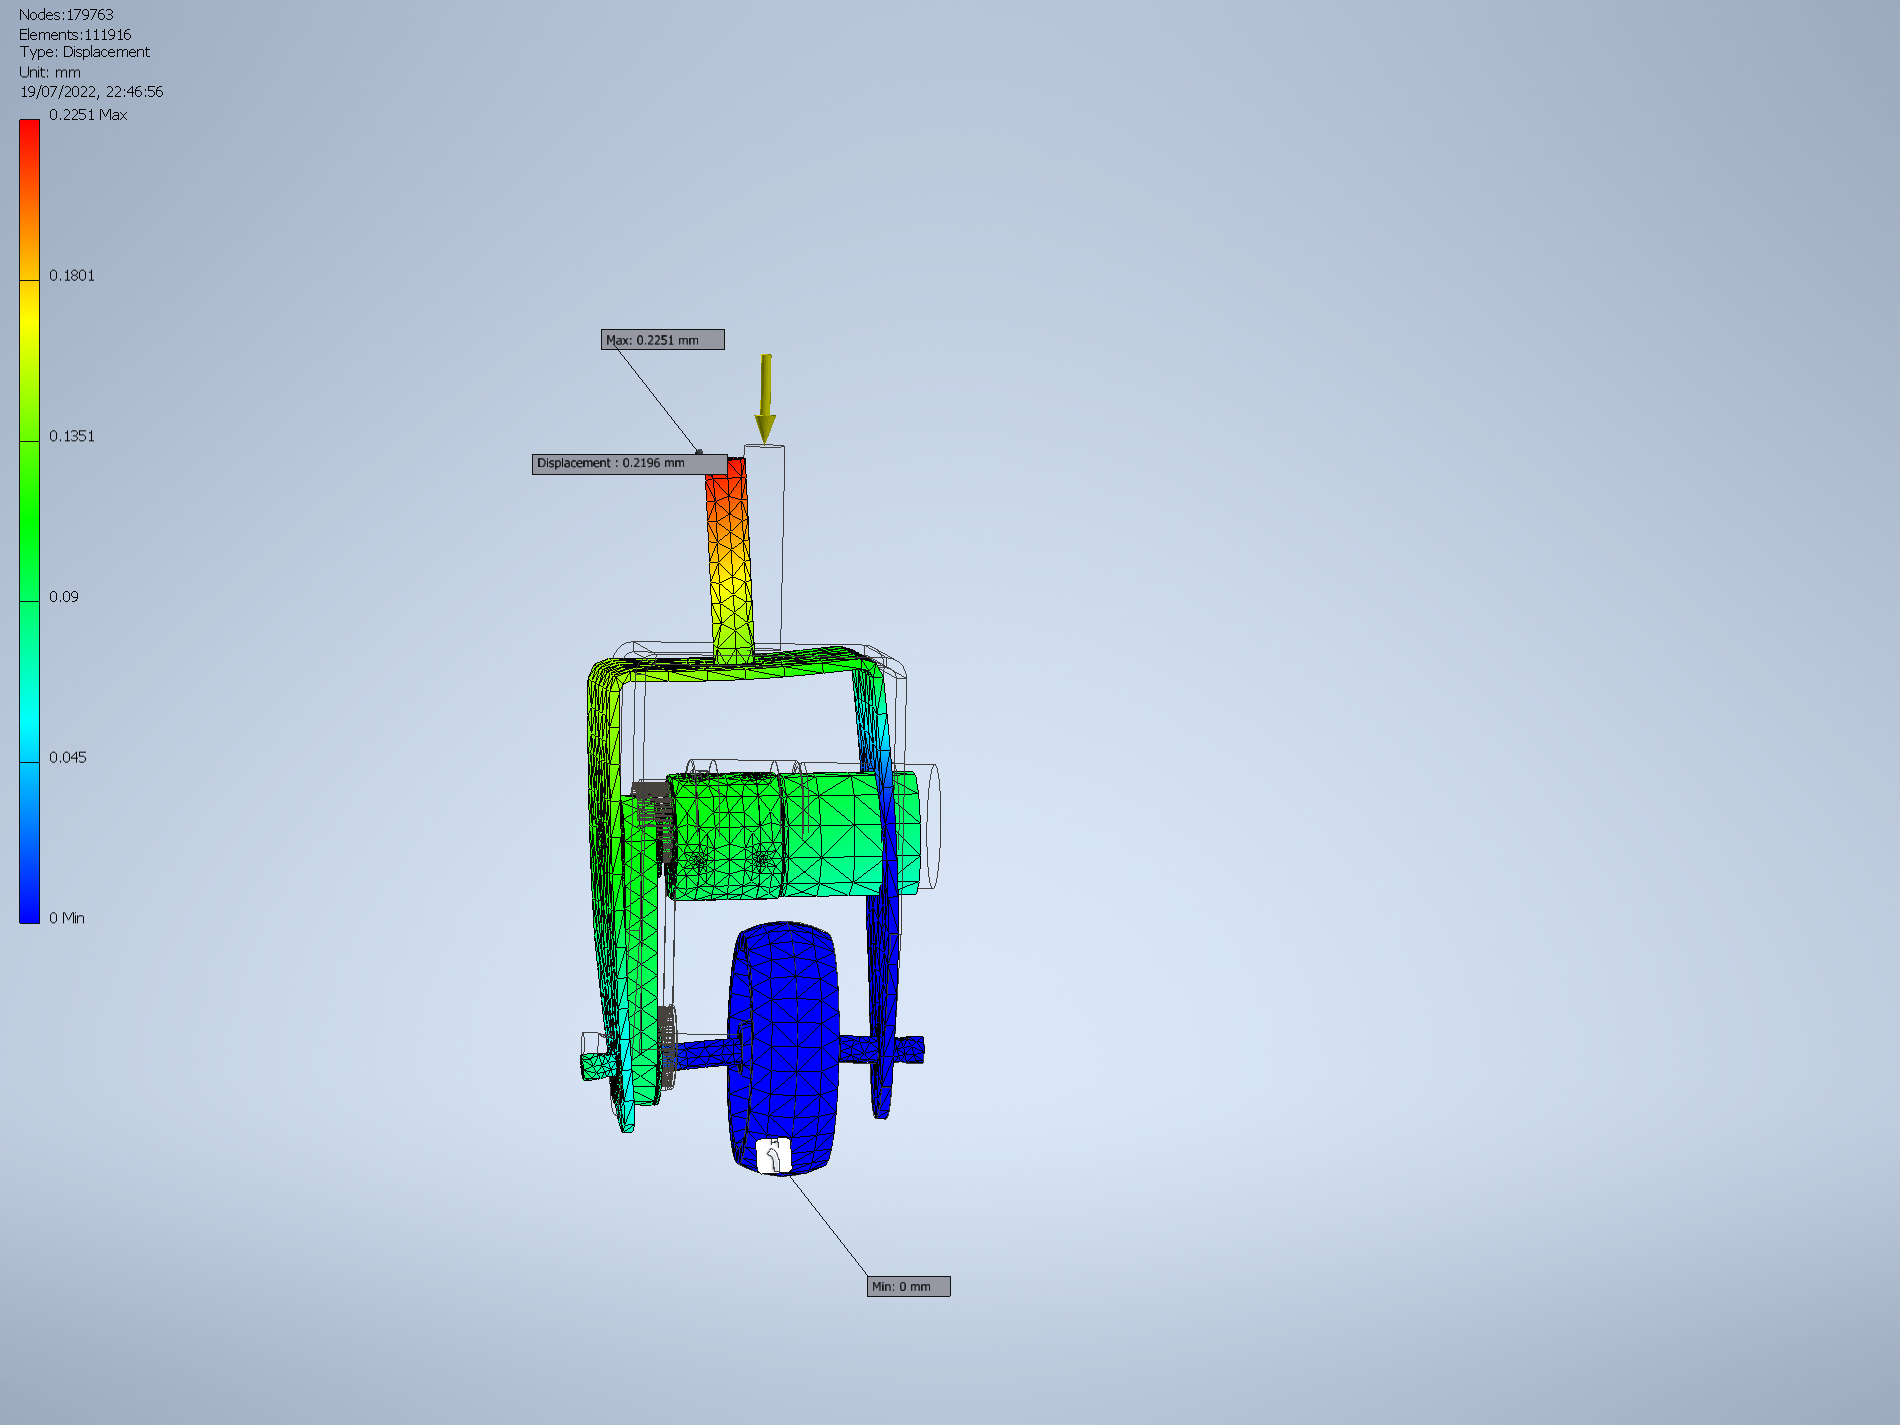
\includegraphics[scale = 0.3]{Figures/WheelFrameDisplacement.png}
%     \caption{Load Displacement on Wheel Frame}
%     \label{fig:wheelframedisplacement}
% \end{figure}

% \section{Motor control analysis}
% TO BE ADDED

\section{Budget}
\begin{table}[H]
  \begin{center}
    \leavevmode
    \hangcaption[Cost Budget]{Cost Budget}
     \begin{tabular}{| l | c | c | c | c | c |}\hline
No. & Item & Quantity & Supplier & Unit Cost & Total cost \\\hline
1 & Satima S2 Motor driver & 4 & Pixel Electric & 500 & 2000 \\\hline
2 & STM32F103C8T6 & 1 & Nerokas & 1000 & 1000 \\\hline
3 & MPU-6050 & 1 & Nerokas & 260 & 260 \\\hline
4 & Esp 12 F & 2 & Nerokas & 300 & 600 \\\hline
5 & Passive components & 1 & Pixel Electric & 1000 & 1000 \\\hline
6 & PCB & 2 & & 500 & 1000 \\\hline
7 & 18650 Lithium Ion Battery & 5 & Pixel Electric & 350 & 1750 \\\hline
8 & DC motor & 8 & Pixel Electric & 1100 & 8800 \\\hline
9 & Motor Bracket & 8 & Pixel Electric & 300 & 2400 \\\hline
10 & Motor shaft and couplings & 4 & Pixel Electric & 200 & 800 \\\hline
11 & Bearing & 4 & Hardware & 100 & 400 \\\hline
12 & V-belt pulley & 16 & Pixel Electric & 150 & 2400 \\\hline
13 & Belt & 8 & Hardware & 200 & 1600 \\\hline
14 & Castor Wheels & 4 & Nerokas & 200 & 800 \\\hline
15 & Steel rods & 5 & Hardware & 60 & 300 \\\hline
16 & Aluminium Sheet & 1 & Hardware & 600 & 600 \\\hline
17 & Fasteners & 1 & Hardware & 500 & 500 \\\hline
18 & Miscalleneous & 1 & & 2600 & 2600 \\\hline
& & & & & \\\hline
& & & & TOTAL & 28810 \\\hline
    \end{tabular}
    \label{table:1}
  \end{center}
\end{table}


\begin{table}[H]
  \begin{center}
    \leavevmode
    \hangcaption[Power Budget]{Power Budget}
     \begin{tabular}{| l | c | c | c | c |}\hline
Component & Voltage (V) & Current (mA) & No. of Components & Power (W) \\\hline
MPU6050 & 3.3 & 4.68 & 1 & 0.015444 \\\hline
ESp32 & 3.3 & 480 & 1 & 1.584 \\\hline
Stm32 & 3.3 & 360 & 1 & 1.188 \\\hline
Led & 3.3 & 120 & 2 & 0.792 \\\hline
DC motor & 12 & 360 & 8 & 34.56 \\\hline
Motor driver & 5 & 43.2 & 1 & 0.216 \\\hline
& & & & 38.355444 \\\hline
    \end{tabular}
    \label{table:1}
  \end{center}
\end{table}


% With a $3.2 Ah$ battery we will be able to run the mobile platform for 1hr without charging. Since we don’t have that, the available battery would be a $2.8 Ah$ battery that would’t raise the cost that much further.

% \begin{equation} \label{totalefficiency}
% \begin{split}
% t & = \frac{2.8}{3.2288}\\
% & = 40 mins 53s
% \end{split}
% \end{equation}

% With a $2.2 Ah$ battery we are now able to run for approximately $40 mins$

  \clearpage
   \lhead{Chapter 5. Conclusion}
    \chapter{Conclusion}
The objective of this project was to design and fabricate a prototype mobile platform with holonomic and omnidirectional motion. This phase only involved the design work which was done conclusively. Design parameters were considered and the design work conducted to accommodate these parameters. The results are in line with the expected outcomes, as evidenced by the detailed CAD drawings produced.
\par
The next step will be implementation and fabrication of the developed design. However, it is expected that during this phase, few modifications and redesigns will have to be made to further optimise the design.
%  \input{Files/Summary}
  \clearpage
%----  Bibliography  ----------------------------------------
\lhead{REFERENCES}
\markright{References}

\addcontentsline{toc}{section}{References}
\bibliographystyle{Bib/IEEEtran}
\bibliography{Bib/References}
  \clearpage
 
 \lhead{APPENDICES}
\markright{APPENDICES}                                
\addcontentsline{toc}{section}{Appendices}                      
\chapter{Appendices}

\section{Time Plan}
% \textbf{Time plan}

\begin{table}[H]
  \begin{center}
    \leavevmode
\hangcaption[Semester 1 Time-plan]{Semester 1 Time-plan}
\begin{tabular}{|l|c|c|c|c|c|c|c|c|c|c|c|} \hline
& \multicolumn{11}{c|}{SEMESTER 1} \\ \hline
\rowcolor{white} Week & 1 & 2 & 3 & 4 & 5 & 6 & 7 & 8 & 9 & 10 & 11 \\ \hline
\rowcolor{white} Project Proposal & & \cellcolor{black} & \cellcolor{black} & \cellcolor{black} & & & & & & & \\ \hline
\rowcolor{white} Continuous Presentation & & & & & \cellcolor{black} & \cellcolor{black} & \cellcolor{black} & \cellcolor{black} & \cellcolor{black} & \cellcolor{black} & \cellcolor{black} \\ \hline
\rowcolor{white} Literature Review & & & & & & \cellcolor{black} & \cellcolor{black} & \cellcolor{black} & \cellcolor{black} & \cellcolor{black} & \cellcolor{black} \\ \hline
\rowcolor{white} Mechanical Design & & & & & & & \cellcolor{black} & \cellcolor{black} & \cellcolor{black} & \cellcolor{black} & \\ \hline
\rowcolor{white} Electrical Design & & & & & & & \cellcolor{black} & \cellcolor{black} & \cellcolor{black} & \cellcolor{black} & \\ \hline
\rowcolor{white} Software Design & & & & & & & & & \cellcolor{black} & \cellcolor{black} & \cellcolor{black} \\ \hline
\rowcolor{white} Material Acquisition & & & & & & & & & & & \cellcolor{black} \\ \hline
\end{tabular}
\label{table:semester1timeplan}
\end{center}
\end{table}

\begin{table}[H]
  \begin{center}
    \leavevmode
\hangcaption[Semester 2 Time-plan]{Semester 2 Time-plan}
\begin{tabular}{|l|c|c|c|c|c|c|c|c|c|c|c|c|c|c|} \hline
& \multicolumn{14}{c|}{SEMESTER 2} \\ \hline
\rowcolor{white} Week & 1 & 2 & 3 & 4 & 5 & 6 & 7 & 8 & 9 & 10 & 11 & 12 & 13 & 14 \\ \hline
\rowcolor{white} Continuos Presentation & \cellcolor{black} & \cellcolor{black} & \cellcolor{black} & \cellcolor{black} & \cellcolor{black} & \cellcolor{black} & \cellcolor{black} & \cellcolor{black} & \cellcolor{black} & & & & & \\ \hline
\rowcolor{white} Literature Review & \cellcolor{black} & \cellcolor{black} & \cellcolor{black} & \cellcolor{black} & \cellcolor{black} & & & & & & & & & \\ \hline
\rowcolor{white} Material Acquisition & \cellcolor{black} & \cellcolor{black} & & & & & & & & & & & & \\ \hline
\rowcolor{white} Mechanical Fabrication & & \cellcolor{black} & \cellcolor{black} & \cellcolor{black} & & & & & & & & & & \\ \hline
\rowcolor{white} Electrical Fabrication & & & \cellcolor{black} & \cellcolor{black} & \cellcolor{black} & & & & & & & & & \\ \hline
\rowcolor{white} Software Fabrication & & & & \cellcolor{black} & \cellcolor{black} & \cellcolor{black} & \cellcolor{black} & & & & & & & \\ \hline

\rowcolor{white} Assembly & & & & & & \cellcolor{black} & \cellcolor{black} & \cellcolor{black} & \cellcolor{black} & & & & & \\ \hline
\rowcolor{white} Testing & & & & & & \cellcolor{black} & \cellcolor{black} & \cellcolor{black} & \cellcolor{black} & \cellcolor{black} & \cellcolor{black} & & & \\ \hline
\rowcolor{white} Demonstration & & & & & & & & & & \cellcolor{black} & \cellcolor{black} & \cellcolor{black} & \cellcolor{black} & \cellcolor{black} \\ \hline
\end{tabular}

\label{table:semester2timeplan}
\end{center}
\end{table}


\section{PCB Designs}

\begin{figure}[H]
    \centering
    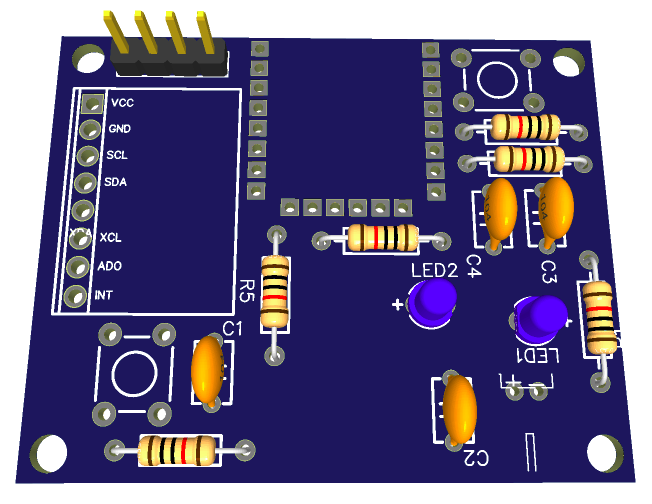
\includegraphics[scale=0.5]{Figures/HMpcb_top.png}
    \caption{Hand Motion Top view of PCB}
    \label{fig:handmotiontopview}
\end{figure}


\begin{figure}[H]
    \centering
    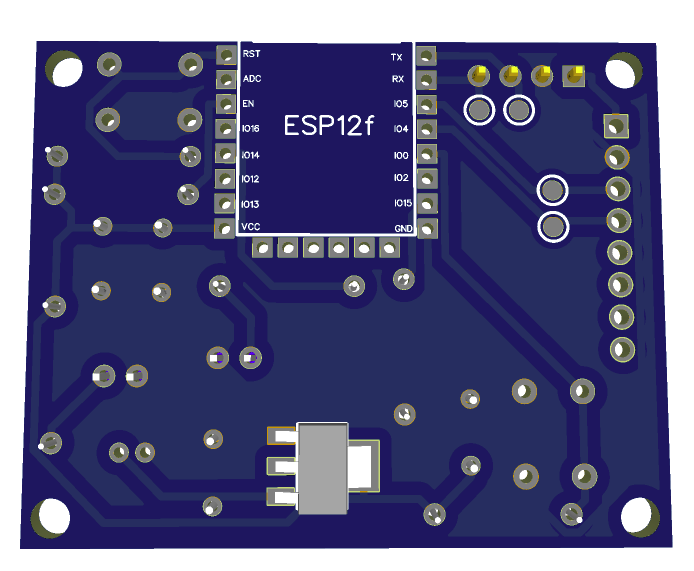
\includegraphics[scale=0.5]{Figures/HMpcb_bottom.png}
    \caption{Hand Motion Bottom view of PCB}
    \label{fig:handmotionbottomview}
\end{figure}


\begin{figure}[H]
    \centering
    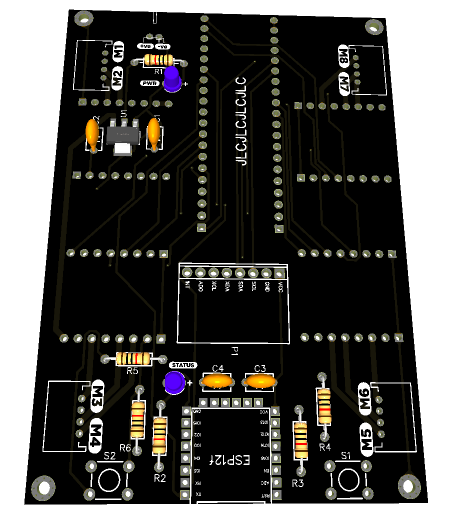
\includegraphics[scale=0.5]{Figures/MPpcb_top.png}
    \caption{Mobile Platform top view}
    \label{fig:mobileplatformtopview}
\end{figure}

\begin{figure}[H]
    \centering
    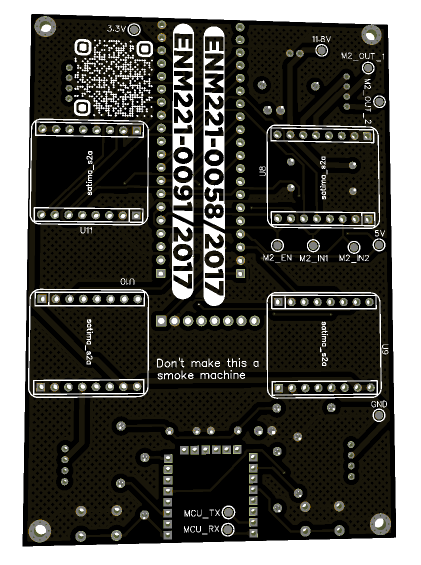
\includegraphics[scale=0.5]{Figures/MPpcb_bottom.png}
    \caption{Mobile Platform bottom view}
    \label{fig:mobileplatformbottomview}
\end{figure}



\section{Production Plans}

\subsection{Mechanical Module}

\begin{enumerate}
    \item Material acquisition. Aluminium sheets to form the platform body and iron rods to construct the chassis will be sourced from a local hardware. Caster wheels will be purchased from an online store.
    \item Once the materials have been acquired, fabrication will commence.
    \item Fabrication techniques to be carried out on the sheet metal that forms the platform body are: sheet metal cutting, sheet metal bending, and boring holes.
    \item The five different parts of the platform will be fabricated using the techniques mentioned above.
    \item Once the different parts have been made, they'll be assembled together using machine screws and nuts.
    \item Fabrication of the chassis will then be conducted by cutting steel rods into the required lengths and joining them using arc welding.
    \item The wheel frames will be fabricated using the same techniques as the parts forming the platform as they are made from sheet metal. 
    \item Once the wheel frames have been made, the motor will be attached using a motor bracket. The wheel and wheel shaft will then be attached allowing the power transmission system of belts and pulley to be attached.
    \item Having assembled the wheel frame components, the frame will be attached to the chassis using a bearing. The platform will then be attached onto the chassis-wheel frame assembly using machine screws.
\end{enumerate}

\subsection{Electrical Module}

\subsubsection{Hand Motion Control PCB}
\begin{enumerate}
    \item Print out the bottom layer onto the Shiny Side of the glossy paper. The copper pads and tracks should be black from figure \ref{fig:HMbottomlayer}.
    \item Sand the copper plate so there is a rough surface for the design to stick to when transferred
    \item Wash the copper with some water and rubbing alcohol and let it dry
    \item Cut out the designs and place them face down on the copper
    \item Run the copper plate with the design face down through a laminator or iron box 5-7 times until the plate is hot 
    \item After running the plate through a laminator or iron place the plate into a cold bath and agitate until the paper floats off
    \item Place the PCB into the etching solution and agitate for 25-30 minutes or until all the copper has dissolved around the design.
    \item Once all the copper is gone rinse it in the water bath, let it dry and use rubbing alcohol to whip off the ink transferred onto the PCB
    \item Drill the holes for DIP components and also mounting holes
    \item Start by placing SMD components and solder them either by hot air gun or hand soldering
    \item Solder DIP components by hand soldering
\end{enumerate}

\begin{figure}[H]
    \centering
    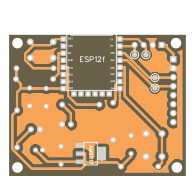
\includegraphics[scale=0.9]{Figures/pcb_bottom.png}
    \caption{Hand motion controller bottom layer}
    \label{fig:HMbottomlayer}
\end{figure}

\subsubsection{Mobile Platform PCB}
For the Mobile Platform PCB it would be great to use using PCB companies such as Gearbox or JLCPCB as it is highly complex for manual fabrication
\begin{enumerate}
    \item Obtain the GitHub repository \cite{gerber_files}.
    \item Submit the Gerber files to respective manufacturer.
\end{enumerate}

\subsection{Software and Control}
The mobile application will be developed using the Flutter framework and Dart language. Flutter applies widgets to construct different features of a window. The basic procedure for Flutter app development is:
\begin{enumerate}
    \item Establish the foundational blocks and classes
    \item Add widgets to the various windows. These widgets can be stateless or stateful widgets depending on whether data/objects change over time.
    \item These widgets are used to add text, images, padding or any other desired frontend features
    \item The application will involve controlling the platform using buttons, so a button widget will be implemented on one window. This widget will be stateful as objects will be changing with time
    \item Once the application has been developed, it will be deployed onto the app stores for the various platforms-android and iOS.
\end{enumerate}
% \appendix
\end{document}
